\label{Chapter4}

\newlength\figureheight
\newlength\figurewidth

\chapter{Experimental Validation}

\section{Scope of Experiments}

The purpose of the experiments is to validate the proposed system as
well as its robustness in various terrains and configurations.
Since the autonomous navigation of the robot is out of the scope of this
thesis, the mapping procedure is only indirectly validated as part of the
SLAM system.
Thus, the main focus of the experiments is the relative and absolute
localization techniques that were developed.

\subsection{Data Collection}

The performed experiments were executed by means of
\textit{Software In the Loop} (SIL) tests using precollected data,
on a computer with a 4\textsuperscript{th} generation Intel\textcopyright\
Core\texttrademark\ i7 processor clocked at $\SI{3.50}{\giga\hertz}$ and
$\SI{16}{\giga B}$ of DDR3 RAM.
The data were collected by the Planetary Robotics Lab team of the European
Space Agency as part of a two week test campaign that took
place in the Minas de San Jose desert in Tenerife, Spain with the aim to
validate the integration of the HDPR rover (Section \ref{hdpr_rover}) and
provide data for future research projects.
The aerial view of the local is presented in Figure \ref{fig:terrain}.

\begin{figure}[h!]
    \centering
    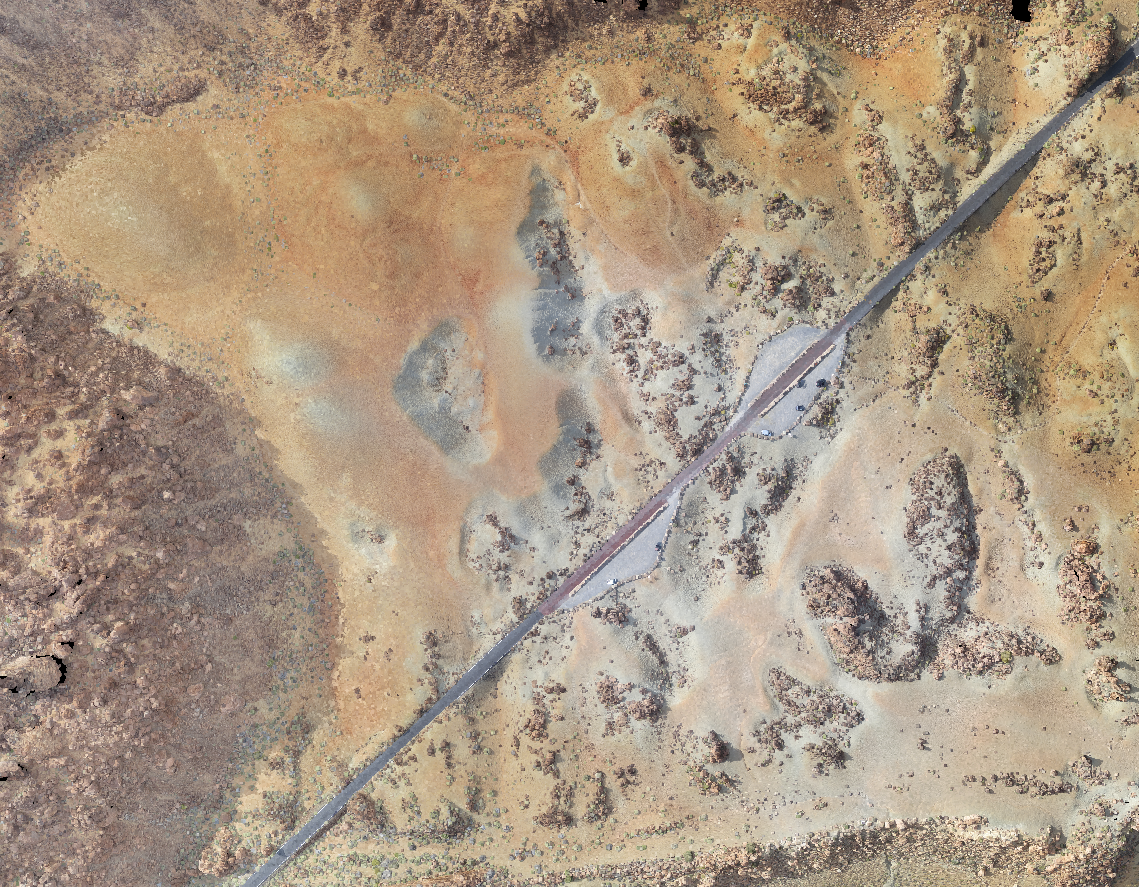
\includegraphics[scale=0.3]{terrain}
    \caption[Aerial view of test field]{
        Aerial view of test field that was reconstructed using drone
        imagery.
    }
    \label{fig:terrain}
\end{figure}

For that reason, the collected dataset contains samples from:
\begin{enumerate*}[label=(\roman*)]
        \item three stereo camera sensors
        \item IMU sensor
        \item point clouds reconstructed from drone imagery
        \item GPS sensor.
\end{enumerate*}
These samples are used both as input to our system and as ground truth
information.

The environment in which the test data were collected, was chosen with
the aim to bear close resemblance to rough planetary terrains,
specifically to the one of Mars.
In particular, various geological properties such as the distribution
and the shape of the rocks is similar to the Martian terrain.

Finally, the speed of the robot in these datasets was chosen to be close
to the $\SI{10}{\cm \per sec}$ value, considering the long-range traverses it was
required to cover.
As such, for the first two experiments, the size of the local map is fixed at
$\SI{20 x 20}{\m}$ and its resolution at $\SI{10}{\cm \per cell}$,
while for the global map we presumed the resolution to be fixed at
$\SI{50}{\cm \per cell}$.
In the third experiment, the performance of our approach is validated against
these parameters, hence they are variable.

\subsection{Metrics} \label{metrics}

To quantify the experimental results and evaluate the outputs of the system,
it is necessary to introduce certain metrics:
\begin{itemize}
    \item \textbf{Mean square error (MSE) of pose graph}:
        This is a straightforward metric for benchmarking SLAM algorithms
        \parencite{Kummerle2009}
        and can be defined as
        \begin{equation}
            \varepsilon_{MSE} (\hat{x}_{1:T}) = \frac{1}{T}
            \sum\limits_{t=1}^T (\hat{x}_t \ominus x_t)^2
        \end{equation}
        where
        $\hat{x}_{1:T}$ is the estimated pose graph,
        $x_{1:T}$ is the ground truth pose graph,
        $T$ is the number of samples and
        $x_i \ominus x_j$ is the distance between two poses.

    \item \textbf{Root mean square deviation (RMSD) of pose graph}:
        Similarly to the MSE metric, this metric expresses the sample
        standard deviation of the differences between the estimated and the
        ground truth poses and can be defined as
        \begin{equation}
            \varepsilon_{RMSD} (\hat{x}_{1:T}) = \sqrt{\frac{1}{T}
            \sum\limits_{t=1}^T (y_t - \varepsilon_{MSE})^2}
        \end{equation}
        where $y_t$ is defined as $\hat{x}_t \ominus x_t$.
\end{itemize}

\section{Experiments on Pose Estimation}

\subsection{Relative Localization Results}

The purpose of this experiment is to test the accuracy of the Pose Estimation
module (see Section \ref{pose_estimation}) and evaluate its capabilities
in a relative localization (short-range) scenario.
To accomplish that, we will carry out each experiment with different parameter
sets with the aim of examining the system's sensitivity as well as finding an
optimal parameter configuration.

The main parameters that we will tune during the experiments are all related
to the particle filter and include
\begin{enumerate*}[label=(\roman*)]
        \item the number of particles used
        \item the resampling frequency
        \item the standard deviation of the Gaussian noise
            added to each particle.
\end{enumerate*}
Finally, the expected error of the estimated pose should ideally be in the
same order of magnitude as the size of one cell of the local map, so as to
ensure that the robot can distinguish the environment's obstacles with
a high-level of certainty.

\begin{figure}[h!]
    \centering
    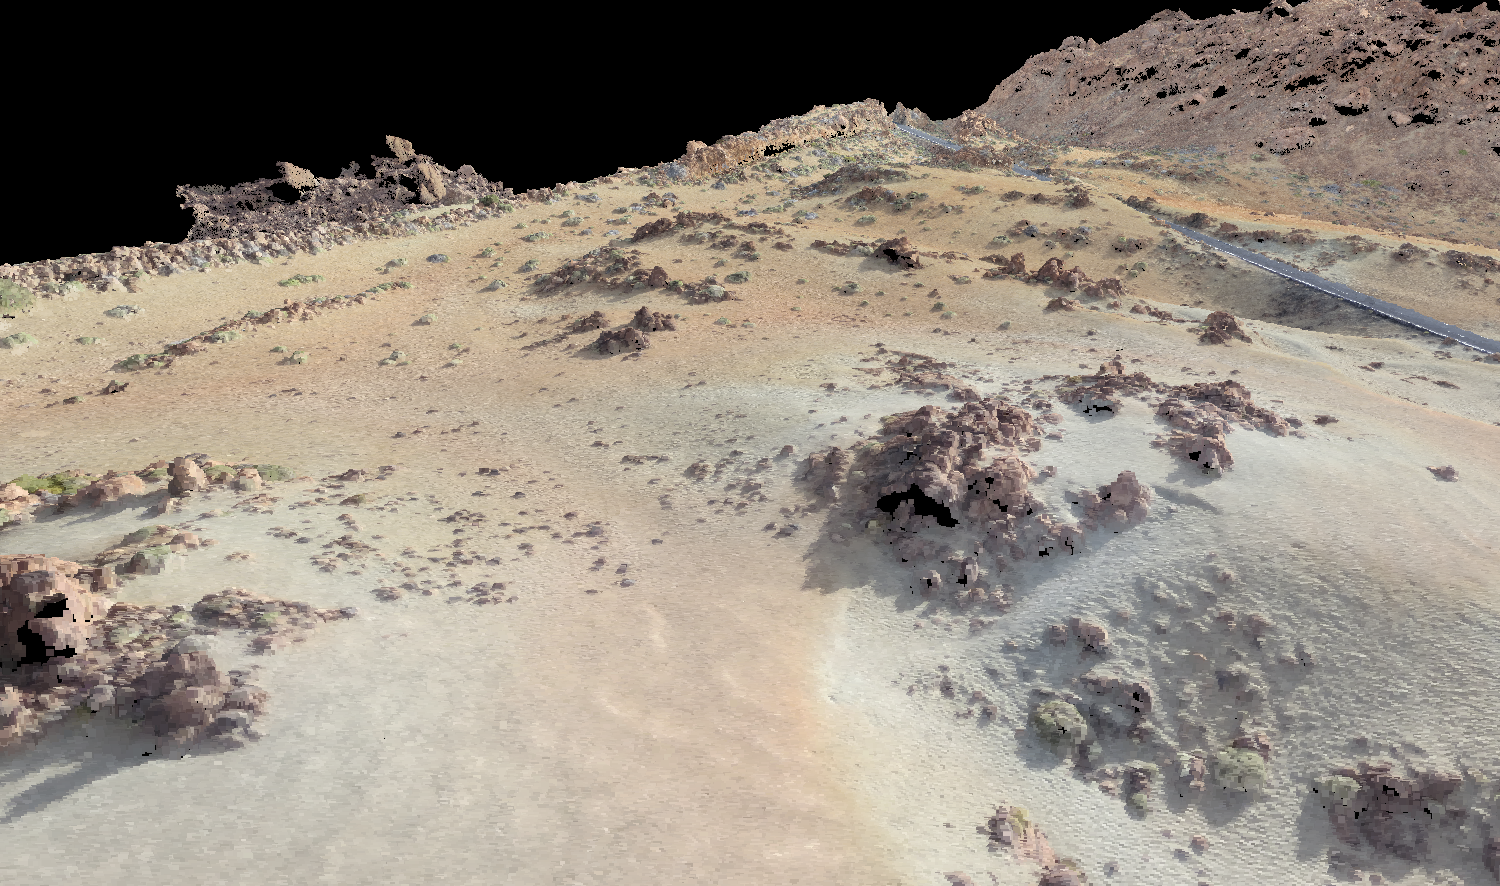
\includegraphics[scale=0.25]{terrain_1}
    \caption[Terrain of first experiment]{
        3D view of the terrain evaluated in the first experiment.
    }
    \label{fig:terrain_1}
\end{figure}

Figure \ref{fig:terrain_1} presents a view of the evaluated terrain of the
first scenario.
The terrain is depicted in the form of one dense point cloud which was
reconstructed from drone imagery.
The bird's eye view in Figures \ref{fig:bird_1_color} and \ref{fig:bird_1_raw}
shows the traverse of the robot in this scenario and compares the ground truth
path, the one from raw visual odometry and the one from the pose estimation.
In contrast to the visual odometry estimate (blue path), the pose estimate
of our system (red path) follows closely the ground truth (black path).
The richness of the terrain in features, which is visible in Figure
\ref{fig:bird_1_real}, is an advantage for relative localization since
the weights of the particles in the particle filter are updated using
scan matching.

\begin{figure}[t]
    \centering
    \begin{subfigure}{0.5\textwidth}
        \centering
        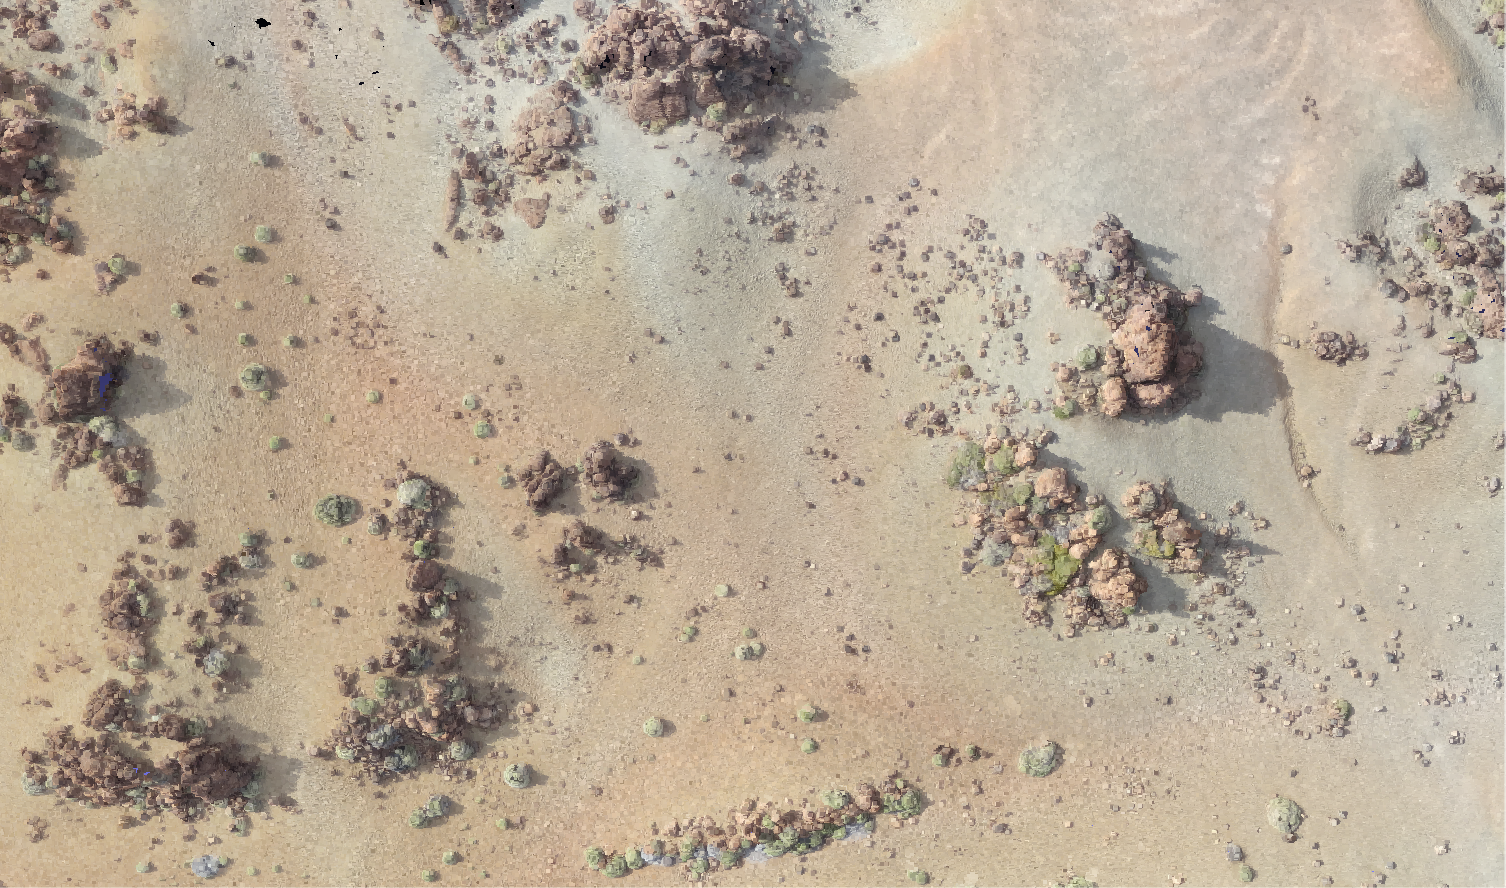
\includegraphics[scale=0.125]{bird_1_real}
        \caption{Point cloud projection}
        \label{fig:bird_1_real}
    \end{subfigure}
    \begin{subfigure}{0.5\textwidth}
        \centering
        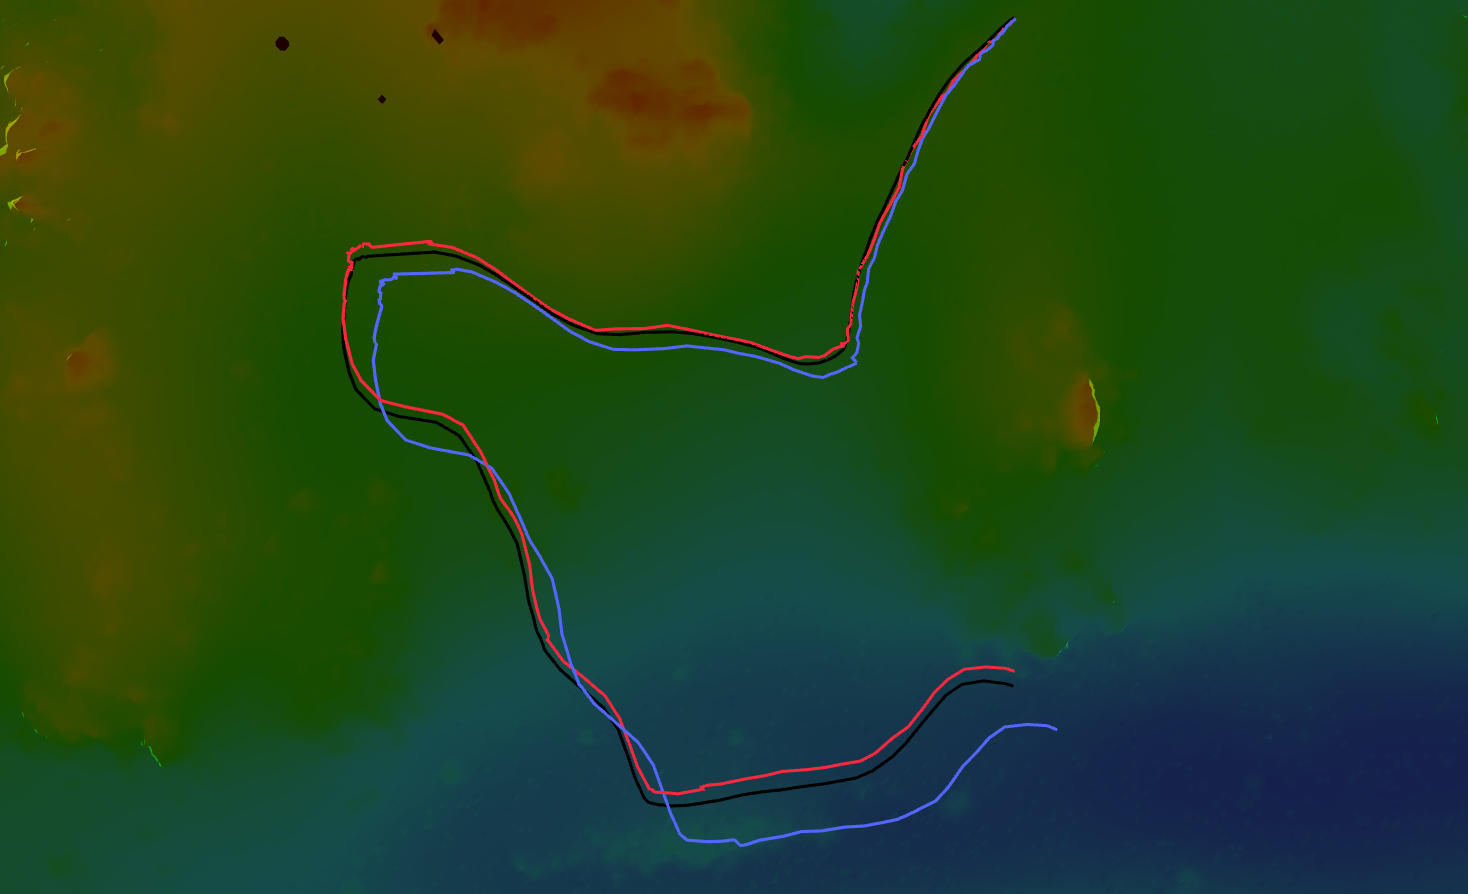
\includegraphics[scale=0.125]{bird_1_color}
        \caption{Global elevation map\\with an elevation colormap}
        \label{fig:bird_1_color}
    \end{subfigure}%
    \begin{subfigure}{0.5\textwidth}
        \centering
        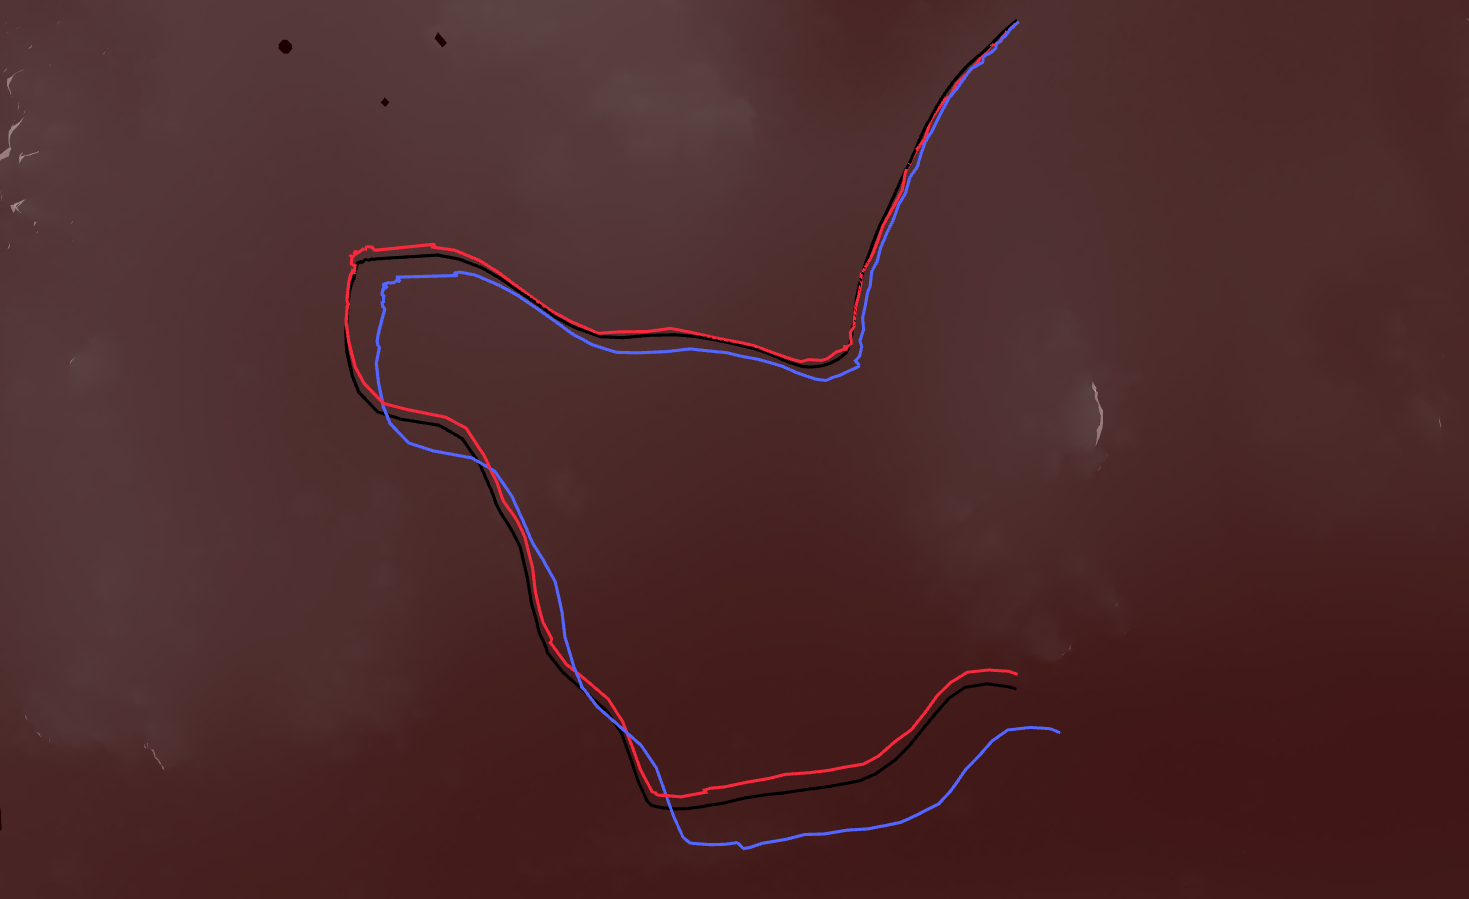
\includegraphics[scale=0.125]{bird_1_raw}
        \caption{Global elevation map\\with raw elevation values}
        \label{fig:bird_1_raw}
    \end{subfigure}
    \caption[Traverse of first experiment]{Orthographic views of the
        environment and the robot's traverses in it. The black, red and
        blue colors correspond to the ground truth, SLAM and visual odometry
        paths accordingly.}
    \label{fig:bird_1}
\end{figure}

In particular, the influence the number of particles used has on the outcome
is shown in the comparison plot in Figure \ref{fig:error_vs_particles}.
We observe that the pose error decreases as we increase the number of particles
used in the particle filter, since the continuous space of the problem
is modelled more effectively.
However, increasing this parameter, brings a proportional increase to
the computation needs for every iteration of the filter.
As it is visible in the plot, a justified choice would be to use 100
particles for a balance of error and processing power.
Furthermore, it is important to notice that the drift in pose ($\SI{20}{\cm}$
in the case of 100 particles), is proportional to the robot's speed
($\SI{10}{\cm \per sec}$ in this experiment).

Regarding the second parameter, the plot in Figure
\ref{fig:error_vs_resampling} represents the same error as the previous plots,
with the difference that the number of particles is fixed to the value of 100
and the resampling frequency is the variable parameter.
It is visible that resampling too often or too rare has an impact on the
pose error.
This is due to the fact that by resampling, the particle population is gathered
near the best belief and as a result other possible solutions are eliminated.

\begin{figure}[h!]
    \centering
    \begin{subfigure}{0.75\textwidth}
        \centering
        \setlength\figureheight{6cm}
        \setlength\figurewidth{10cm}
        % This file was created by matplotlib2tikz v0.6.15.
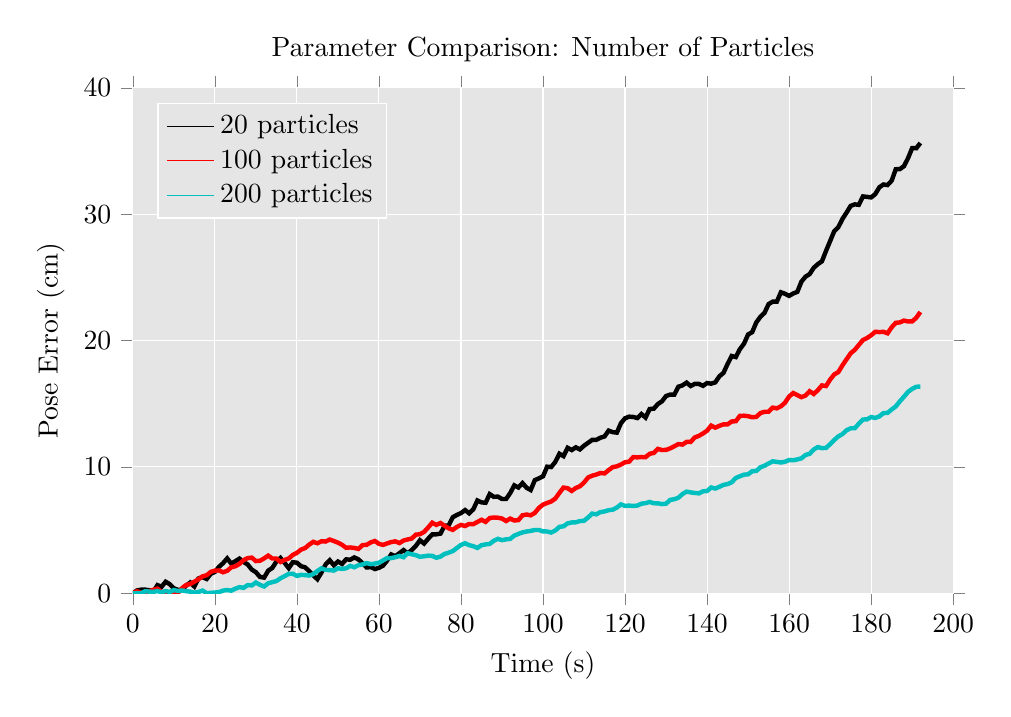
\begin{tikzpicture}

\definecolor{color0}{rgb}{0,0.75,0.75}

\begin{axis}[
title={Parameter Comparison: Number of Particles},
xlabel={Time (s)},
ylabel={Pose Error (cm)},
xmin=0, xmax=200,
ymin=0, ymax=40,
width=\figurewidth,
height=\figureheight,
tick align=outside,
tick pos=both,
xmajorgrids,
x grid style={white},
ymajorgrids,
y grid style={white},
axis line style={white},
axis background/.style={fill=white!89.803921568627459!black},
legend style={at={(0.03,0.97)}, anchor=north west, draw=white, fill=white!89.803921568627459!black},
legend entries={{20 particles},{100 particles},{200 particles}},
legend cell align={left}
]
\addlegendimage{no markers, black}
\addlegendimage{no markers, red}
\addlegendimage{no markers, color0}
\addplot [ultra thick, black]
table {%
0 0
1 0.221275467285065
2 0.283236011481664
3 0.288259883639869
4 0.24005721981802
5 0.123194324335208
6 0.64227586529811
7 0.50950825096868
8 0.909862308820304
9 0.720138179974689
10 0.390336716658979
11 0.267222731593722
12 0.256367873942256
13 0.604496280195007
14 0.850466116117319
15 0.535957176111004
16 1.17185055953395
17 1.27188527609326
18 1.12800363499572
19 1.53968911567716
20 1.68467852268559
21 2.09074920928784
22 2.38346096310586
23 2.75734756317857
24 2.3439720089918
25 2.53926344276542
26 2.74031916752099
27 2.47689578798731
28 2.27770827456999
29 1.87175395283667
30 1.66464479958335
31 1.29212512581763
32 1.23642176707551
33 1.78527359382804
34 2.00371389635228
35 2.50954850519101
36 2.79580747247973
37 2.40563583744804
38 1.98817494304728
39 2.45832283818954
40 2.41884615311573
41 2.14128179105048
42 2.05223529990283
43 1.74400977369496
44 1.42157123035973
45 1.10941404686447
46 1.64740291267012
47 2.27651121043169
48 2.61198489019321
49 2.21982890694873
50 2.51097398464712
51 2.32131450717707
52 2.68261417875233
53 2.65383558532601
54 2.83399031539634
55 2.6808959419985
56 2.37972602417066
57 2.04030802825984
58 2.06802158744433
59 1.91993559519338
60 2.0126652579686
61 2.18481741677879
62 2.59205403129238
63 3.07070255565471
64 2.9283516933866
65 3.17370073513823
66 3.41706276462247
67 3.16110314205998
68 3.41992413128208
69 3.74655240177972
70 4.19225714582931
71 3.93407337338655
72 4.31471664720745
73 4.65599988467862
74 4.66449959782519
75 4.71970818018142
76 5.33809613188595
77 5.37170909980747
78 6.01583520075567
79 6.19818856107466
80 6.34428113937773
81 6.58155685751761
82 6.32929408033819
83 6.63937719391216
84 7.34192012793726
85 7.19351068826223
86 7.16265584504585
87 7.84619933694429
88 7.63405394050247
89 7.64764238897803
90 7.46169755434128
91 7.45996442886437
92 7.9277619179694
93 8.53828837487015
94 8.3719946071987
95 8.71710818104912
96 8.34767686396481
97 8.17215667653221
98 8.94942980493243
99 9.0930912448854
100 9.25665955969415
101 10.0162278352991
102 9.98860380850638
103 10.3967676213816
104 11.0419254562774
105 10.8530995942226
106 11.5122795423599
107 11.3347324207578
108 11.5474154848702
109 11.3832905058985
110 11.6799720960744
111 11.9097221364012
112 12.1392279159714
113 12.1431667276411
114 12.3099837601932
115 12.410132832305
116 12.8715061996322
117 12.7515799200313
118 12.7116407915538
119 13.4580131767435
120 13.8491978413642
121 13.9762722092058
122 13.9532531525485
123 13.8678695691263
124 14.1822444603177
125 13.9071465850899
126 14.5828777463424
127 14.607701936195
128 14.9742646630127
129 15.1907480538657
130 15.6100647948631
131 15.7247925226392
132 15.7186541117421
133 16.3477264735683
134 16.454786344381
135 16.6708887919105
136 16.4028355943374
137 16.5743818499265
138 16.5675305519801
139 16.419188313567
140 16.6384056459799
141 16.5887106675688
142 16.6923894985961
143 17.1703547026931
144 17.4435100764463
145 18.1470434713598
146 18.7794155165855
147 18.6946819157778
148 19.3193358458556
149 19.7514914963871
150 20.4811346960366
151 20.667602025894
152 21.4354476983997
153 21.8829048387394
154 22.1910431754188
155 22.888706148098
156 23.0757535995025
157 23.0826309830089
158 23.8205028592497
159 23.7040490282308
160 23.5366777552433
161 23.7273854932021
162 23.8532151919259
163 24.6647306208241
164 25.0560626214709
165 25.2590463832891
166 25.7600006574152
167 26.048773529415
168 26.2757397292951
169 27.098213756413
170 27.8741164291256
171 28.659564023246
172 28.9796930867021
173 29.6268267035997
174 30.1267482766181
175 30.6562288442046
176 30.7789039942204
177 30.7417931019391
178 31.407337603908
179 31.3726432037337
180 31.3291129387772
181 31.5921756539376
182 32.1302166360578
183 32.3528124249666
184 32.3076326931206
185 32.6554397798917
186 33.5604719343999
187 33.5716325058484
188 33.8032775838931
189 34.4395607516101
190 35.236822059255
191 35.2206791063638
192 35.6357206214822
};
\addplot [ultra thick, red]
table {%
0 0
1 0.159935556346842
2 0.0458095759658287
3 0.0840886058631565
4 0.160763054533741
5 0.273412159134529
6 0.362488875749649
7 0.112226331939905
8 0.0191139944878066
9 0.0816273758564361
10 0.0131083991961984
11 0.029466546403391
12 0.40765505647619
13 0.654025611689312
14 0.730246234750432
15 0.916618953928916
16 1.10924351080036
17 1.33675911680249
18 1.42441686345835
19 1.69099912788567
20 1.79175137800724
21 1.80400830938948
22 1.66251801818832
23 1.77512124707824
24 2.05528219877006
25 2.13291511133442
26 2.321257906011
27 2.62064343557571
28 2.7795484879304
29 2.81974322933337
30 2.54867020709085
31 2.57162177174894
32 2.75565133776691
33 2.97785865343797
34 2.74944414599111
35 2.74841889459765
36 2.47708935271412
37 2.63597105782224
38 2.75166212459774
39 3.03431411723827
40 3.19591428626382
41 3.45395464489952
42 3.57693464647281
43 3.85053007714457
44 4.07038012393075
45 3.95480414735672
46 4.11762080139084
47 4.09210486800269
48 4.24903202585971
49 4.1361059084061
50 4.00522331808708
51 3.83717351257513
52 3.59911393680789
53 3.62500797499391
54 3.58493633860171
55 3.51216326828598
56 3.81031578788626
57 3.83150149257737
58 4.02670458567878
59 4.13809872065115
60 3.91312580168342
61 3.82697747464603
62 3.94284852237389
63 4.05349306503138
64 4.10509877251611
65 3.97237280402713
66 4.17106606614425
67 4.2598634214947
68 4.33027972684033
69 4.63812098728964
70 4.67199796537047
71 4.8548082199671
72 5.20556019671771
73 5.58336037431889
74 5.41227810184391
75 5.56044423540978
76 5.33993243180194
77 5.14069512972942
78 5.01946696014079
79 5.24922545392262
80 5.41094462819385
81 5.32153495618899
82 5.4823242143079
83 5.46864318454501
84 5.64137688825727
85 5.81223481931553
86 5.64577809230002
87 5.95364717613265
88 5.9968601342492
89 5.9776547646192
90 5.9134403910347
91 5.71770099461532
92 5.9100696748241
93 5.75724757372084
94 5.78981448414988
95 6.16954661564645
96 6.23152990482817
97 6.1682658442305
98 6.36017556162752
99 6.75154274358601
100 7.01352841604884
101 7.1485179942046
102 7.26404291693646
103 7.49461977832378
104 7.94790205134065
105 8.3643366638633
106 8.31367031782169
107 8.09918368662443
108 8.33217880452605
109 8.46688974550028
110 8.75957599749348
111 9.16490852193891
112 9.3049829733115
113 9.39589907608105
114 9.51726925199251
115 9.48271518858532
116 9.74760751364742
117 9.98151917527905
118 10.0451683452547
119 10.186861913297
120 10.3668900672634
121 10.4223416721838
122 10.7758628869418
123 10.7556939505921
124 10.7839931183652
125 10.7702578273704
126 11.0368279872173
127 11.1086810353969
128 11.4253547617186
129 11.3352624413511
130 11.3455550490804
131 11.4646790170615
132 11.6313518387882
133 11.8050704309764
134 11.7661837866285
135 11.9786005427229
136 11.9763234862531
137 12.3340688302837
138 12.4563237053618
139 12.6483010043573
140 12.8665918747764
141 13.2668972260576
142 13.105972085477
143 13.2527885219443
144 13.3678784249506
145 13.3697350046675
146 13.5952358674915
147 13.6169776196847
148 14.035949407449
149 14.0549207871238
150 14.0120198569208
151 13.9334842518298
152 13.9572410767516
153 14.2607408296282
154 14.3606352888537
155 14.3702459680046
156 14.6914217553308
157 14.6341139454471
158 14.7962986029131
159 15.081563799034
160 15.5697316962165
161 15.8451986307207
162 15.6856095654309
163 15.5230123308348
164 15.6461859549573
165 15.9879571946045
166 15.7735348902736
167 16.0707557553942
168 16.4509966974118
169 16.399350783432
170 16.910791191874
171 17.3179322724094
172 17.5035530418401
173 18.0393457690169
174 18.5166888597458
175 18.9915832723194
176 19.2631755672427
177 19.6554209625895
178 20.0437417338883
179 20.2012518989116
180 20.4223331392501
181 20.6946370977686
182 20.6710246461494
183 20.6923660180652
184 20.5742402920741
185 21.0505919406573
186 21.4055714583677
187 21.4374459576732
188 21.5801210163509
189 21.5101664630108
190 21.5157015290175
191 21.8031494154491
192 22.2590239760641
};
\addplot [ultra thick, color0]
table {%
0 0
1 0.00361471505193553
2 0.000530381241491621
3 0.161254967988251
4 0.128731254088338
5 0.108999090472427
6 0.178704379969392
7 0.0726186415556864
8 0.181700631002427
9 0.0982091332008208
10 0.257910625758513
11 0.18269036156079
12 0.219250973553277
13 0.163156812070203
14 0.127985691300471
15 0.0451198605778245
16 0.102965170491833
17 0.2120439203088
18 0.0106641926097425
19 0.0297454619604669
20 0.0570304843569242
21 0.0924527520953649
22 0.208717034984198
23 0.25845471430241
24 0.201680189503492
25 0.365481008557272
26 0.486085608467989
27 0.427221415064352
28 0.649234294836356
29 0.617980473832794
30 0.852619107634408
31 0.664287539595942
32 0.536675342118031
33 0.789114175879052
34 0.881485908629975
35 0.966104691248484
36 1.18730169778077
37 1.34971812699315
38 1.53136836770027
39 1.54526806360309
40 1.37375271717329
41 1.45373167170819
42 1.4364588420991
43 1.39990612084897
44 1.51618679530693
45 1.76432159823824
46 1.97159754520388
47 1.84521697288315
48 1.83360831812528
49 1.79342527752528
50 1.97430082378588
51 1.93254355916105
52 1.97414189702298
53 2.1667058451988
54 2.05894766161515
55 2.22223705189179
56 2.27829363349054
57 2.38612020296259
58 2.3048171700543
59 2.34932602079422
60 2.41396385962167
61 2.59276260201708
62 2.78897598773625
63 2.78103547293691
64 2.85382026962126
65 2.9553235822689
66 2.85004588410527
67 3.16810447828987
68 3.0873843191722
69 3.01526018935319
70 2.88263607493435
71 2.92777159625986
72 2.97421334184389
73 2.96243589004766
74 2.80592023392333
75 2.90021436457027
76 3.11073843683418
77 3.21230622996918
78 3.33450662118875
79 3.58162480511858
80 3.82164583756433
81 3.95684662499164
82 3.80639961216867
83 3.72706150022347
84 3.58652474823679
85 3.80348859218021
86 3.86471559406116
87 3.90452131170832
88 4.15303226705797
89 4.30560900511285
90 4.20376763399635
91 4.26404038807697
92 4.30392636307526
93 4.56087488832189
94 4.69872555778223
95 4.81524725410293
96 4.88781643578357
97 4.93577195150726
98 5.00882458699346
99 5.00816031943098
100 4.90043104408654
101 4.88845881386522
102 4.80620919341178
103 4.96906043673939
104 5.25390431936644
105 5.30009270138697
106 5.5315329972214
107 5.60257959507081
108 5.61713356846543
109 5.71580586456705
110 5.73672178997937
111 6.00285507304917
112 6.30404906035013
113 6.24617726878152
114 6.42358828742821
115 6.47435706165644
116 6.57602932957808
117 6.61360048400199
118 6.78436308225782
119 7.03110112920373
120 6.91289116346065
121 6.94067505209205
122 6.90577572925083
123 6.94050578195093
124 7.08810390497424
125 7.13393361646521
126 7.22570905320239
127 7.12234430810341
128 7.11640326461755
129 7.05927180799289
130 7.08742697287364
131 7.38900872704062
132 7.44076119231491
133 7.56389658086898
134 7.84972621309571
135 8.04405272865735
136 7.98390343266809
137 7.93813041994009
138 7.90383684936688
139 8.06672686682584
140 8.0931832710696
141 8.37147761103579
142 8.28870868068
143 8.42437942199872
144 8.5795069019368
145 8.64170154546991
146 8.78626525348373
147 9.12211076325171
148 9.26206723319242
149 9.3853522945624
150 9.41401948270264
151 9.66052247374155
152 9.68152071057911
153 9.96834103044044
154 10.0946217648387
155 10.271171900045
156 10.4408523241532
157 10.3994512632777
158 10.3481672716356
159 10.4103957055335
160 10.5447448041654
161 10.525195290301
162 10.5921753656114
163 10.6805378117938
164 10.9453496711215
165 11.0380233789345
166 11.3770277418961
167 11.5670194890254
168 11.4898454518976
169 11.5020504291133
170 11.8013167203996
171 12.1358656164767
172 12.4126993304973
173 12.5973142285151
174 12.8965609453624
175 13.0552304828648
176 13.0650749926276
177 13.4226458822191
178 13.7489206476252
179 13.7654528319067
180 13.9486290890146
181 13.8750793848092
182 13.9985043504883
183 14.258158241056
184 14.2763339257
185 14.5447712424274
186 14.7863849847097
187 15.1913145890867
188 15.554106342059
189 15.9412525006319
190 16.1774812080119
191 16.3428659636106
192 16.3559045751863
};
\end{axis}

\end{tikzpicture}
        \caption{}
        \label{fig:error_vs_particles}
    \end{subfigure}
    \begin{subfigure}{0.75\textwidth}
        \centering
        \setlength\figureheight{6cm}
        \setlength\figurewidth{10cm}
        % This file was created by matplotlib2tikz v0.6.15.
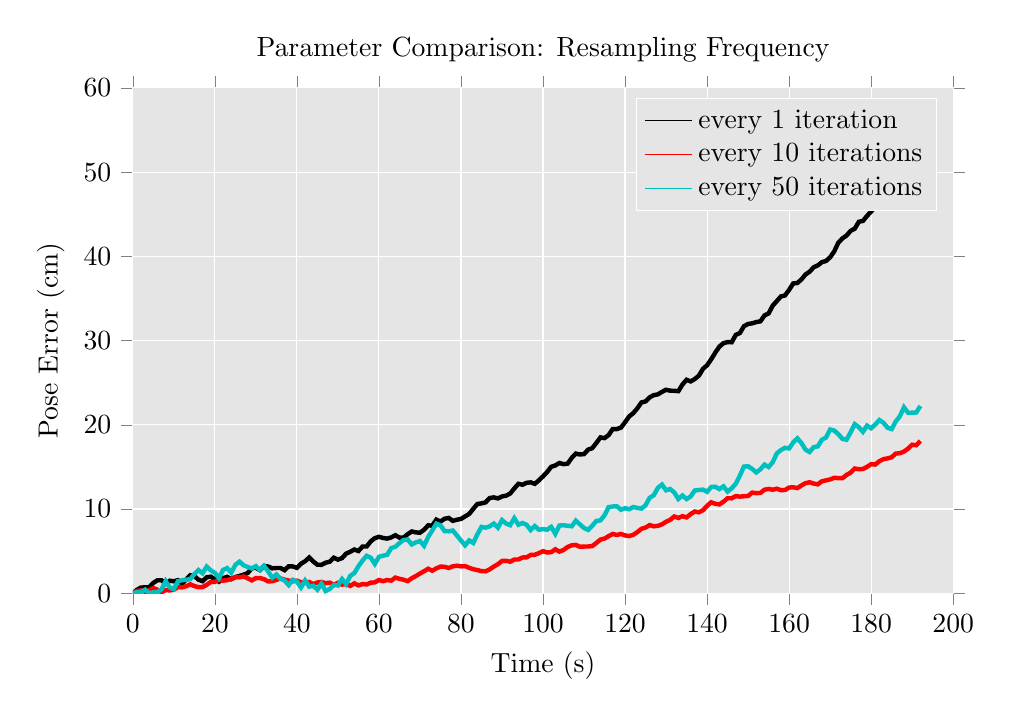
\begin{tikzpicture}

\definecolor{color0}{rgb}{0,0.75,0.75}

\begin{axis}[
title={Parameter Comparison: Resampling Frequency},
xlabel={Time (s)},
ylabel={Pose Error (cm)},
xmin=0, xmax=200,
ymin=0, ymax=60,
width=\figurewidth,
height=\figureheight,
tick align=outside,
tick pos=both,
xmajorgrids,
x grid style={white},
ymajorgrids,
y grid style={white},
axis line style={white},
axis background/.style={fill=white!89.803921568627459!black},
legend entries={{every 1 iteration},{every 10 iterations},{every 50 iterations}},
legend style={draw=white, fill=white!89.803921568627459!black},
legend cell align={left}
]
\addlegendimage{no markers, black}
\addlegendimage{no markers, red}
\addlegendimage{no markers, color0}
\addplot [ultra thick, black]
table {%
0 0
1 0.406198986478148
2 0.685016922140314
3 0.692737183470917
4 0.721698746475873
5 1.23463326514222
6 1.54305050386074
7 1.54147384628651
8 1.1287437563075
9 1.48948142790457
10 1.42276811671587
11 1.55620504745392
12 1.1320824008549
13 1.6328054098618
14 2.13946520204155
15 2.04518920568443
16 1.61347606590852
17 1.43522408027539
18 1.89327016243687
19 1.96858611617375
20 1.64723226803015
21 1.36834735484551
22 1.79942048454682
23 1.9482080068309
24 1.67233779250134
25 1.91932393108407
26 2.05524730451229
27 2.20767715171374
28 2.39731586383221
29 2.96169329037537
30 3.03047072494907
31 2.74489341109166
32 3.23230040066384
33 3.17594498214744
34 2.95880506449785
35 3.00262667182811
36 2.99774447995714
37 2.75028114537336
38 3.20590517429002
39 3.18364821848116
40 3.01426985708579
41 3.51429903954213
42 3.80191177910537
43 4.24374355325379
44 3.76388637781684
45 3.38454938955534
46 3.37851287473816
47 3.62267488326649
48 3.75077403966296
49 4.21438092515273
50 3.99267758979942
51 4.17359698864457
52 4.70458963637373
53 4.92430978019184
54 5.19545435823653
55 5.0159414673874
56 5.54637938529152
57 5.55424203987958
58 6.15932011589112
59 6.54314983947193
60 6.70333699890362
61 6.56717333840685
62 6.48888491897688
63 6.63152164802847
64 6.88936168881749
65 6.60479013797743
66 6.59396258574101
67 7.00993206723238
68 7.33304373960273
69 7.23187555521078
70 7.18242316093635
71 7.54292738323405
72 8.05843900778189
73 8.02758261796706
74 8.73906725884595
75 8.50456222990745
76 8.84648091959684
77 8.94159301175197
78 8.60095770117754
79 8.73091625656062
80 8.82164097749626
81 9.12395451194248
82 9.41978412970761
83 10.026548897847
84 10.6004857997479
85 10.6707565353538
86 10.7939291442093
87 11.3070347074127
88 11.3836343765273
89 11.2591837073136
90 11.4887025942412
91 11.5901131771041
92 11.8408592195988
93 12.4410690432928
94 12.9931055563051
95 12.884239058263
96 13.1136859548283
97 13.1621967531476
98 12.9955955231865
99 13.4078920652958
100 13.8758886769166
101 14.3882589055046
102 15.0157583577483
103 15.169907921748
104 15.4689304589835
105 15.3260253327252
106 15.3886279857664
107 16.0705829711438
108 16.5832238517944
109 16.4726860735252
110 16.5234024712283
111 17.0513930828967
112 17.2266693689533
113 17.8399121277825
114 18.5025166027769
115 18.4190865472945
116 18.7813794791892
117 19.4968044637489
118 19.4940189086537
119 19.6594022788615
120 20.3035426057616
121 20.9887400076541
122 21.3818087906986
123 21.9579331810454
124 22.6560723235941
125 22.7739192256879
126 23.2588369436327
127 23.5182634415758
128 23.6136883017947
129 23.9087342959733
130 24.154518573049
131 24.0503948726874
132 24.0369993913609
133 23.9925082618246
134 24.7841354308156
135 25.3423412514935
136 25.1532072901194
137 25.4342355710751
138 25.8335597832301
139 26.6464386716143
140 27.0653675964988
141 27.7735238521599
142 28.5681840792803
143 29.2775147270817
144 29.6959192310298
145 29.8221856116845
146 29.8001537537629
147 30.6771236558233
148 30.8946792075143
149 31.710425046134
150 31.9690827547475
151 32.0468771151291
152 32.1989793296566
153 32.2824655338836
154 32.9839204623398
155 33.2254757497382
156 34.1434340516444
157 34.6869588884028
158 35.2388904338277
159 35.3567702676745
160 36.0177788513313
161 36.7811943476874
162 36.8282480846606
163 37.2572353259078
164 37.8464804807767
165 38.1759849745191
166 38.7063611567029
167 38.9267920564359
168 39.3113523259026
169 39.4469998395018
170 39.8877547034063
171 40.5916431841307
172 41.6209812305952
173 42.1300515835178
174 42.4662972992114
175 43.031642444094
176 43.2845575097475
177 44.1042203161934
178 44.2072380134832
179 44.8039522720093
180 45.3131520916089
181 45.905042549324
182 45.8044230502413
183 46.0243364090137
184 46.2365976563449
185 46.459195451128
186 46.9670570398638
187 47.6488185997884
188 48.2017456405409
189 49.0225468032041
190 49.7136511122967
191 50.2985408002155
192 50.528185566811
};
\addplot [ultra thick, red]
table {%
0 0
1 0.266063286034632
2 0.363714792730437
3 0.175829842061137
4 0.349771187069945
5 0.624459802425644
6 0.421674925557472
7 0.133125173930802
8 0.36977952679051
9 0.342086276070564
10 0.424582459837136
11 0.739068586362339
12 0.696151077070587
13 0.83096686047733
14 1.05977392918058
15 0.858319178701951
16 0.720687190927617
17 0.737573238848485
18 0.999496187194419
19 1.33655102686123
20 1.34720546953488
21 1.59589223300048
22 1.50013331758343
23 1.55321189409743
24 1.70881753311825
25 1.93782773953266
26 1.88797566090087
27 1.99277183414052
28 1.77835857248429
29 1.52842892861293
30 1.80321626033692
31 1.81008955988835
32 1.66982599332719
33 1.40137029076609
34 1.42954797023367
35 1.5754168044184
36 1.76068896795704
37 1.61198299948591
38 1.50600277516215
39 1.41909211907251
40 1.49591797569885
41 1.31062884860629
42 1.33090689051614
43 1.34180641026505
44 1.08606750276472
45 1.28283715275594
46 1.3432304373597
47 1.19773803890486
48 1.25722196711716
49 1.00535641249088
50 1.23729956430948
51 1.02495482326097
52 1.09990347270338
53 0.876721908976098
54 1.17513601052529
55 0.936647447060198
56 1.08680615180723
57 1.04384136332587
58 1.25618508531157
59 1.2930004591411
60 1.5706967973238
61 1.43418845091583
62 1.5751858850117
63 1.49528162729694
64 1.85950832271678
65 1.71528529463389
66 1.60905743775667
67 1.4454589078338
68 1.77685699416571
69 2.04347109889072
70 2.3406118739616
71 2.61213257069211
72 2.90595454304545
73 2.6782568419172
74 2.9513464961249
75 3.16419379260671
76 3.14685882697593
77 2.99587063154161
78 3.19541690113474
79 3.27173293183559
80 3.19651529209507
81 3.21781926016739
82 3.02403128563506
83 2.85039526378125
84 2.75753411131811
85 2.62597471977156
86 2.60691773064779
87 2.8356692960042
88 3.16645382929236
89 3.44610510168893
90 3.83527609734858
91 3.85520901338764
92 3.74734673121687
93 4.00326650251546
94 4.01489069551452
95 4.24685158229927
96 4.26328859885806
97 4.55032759056344
98 4.56885666738056
99 4.76334276409337
100 4.99986340798858
101 4.83796463173252
102 4.87664307499735
103 5.22046211077534
104 4.94344994512081
105 5.13708166316887
106 5.49506373211306
107 5.69432769471989
108 5.73861368967698
109 5.519670190135
110 5.54660175408973
111 5.55349881165422
112 5.60094310137764
113 5.97312744024343
114 6.37021732829268
115 6.49736373122766
116 6.78416864684926
117 7.04205540452804
118 6.92298242056059
119 7.04165147617447
120 6.86904362298161
121 6.78855818517774
122 6.94206871850499
123 7.25741085936205
124 7.65513653182405
125 7.80190779014427
126 8.09163788116545
127 7.94925955001801
128 8.00489528473665
129 8.17708499773435
130 8.48421234896405
131 8.71696886010417
132 9.11316196162681
133 8.94312507358715
134 9.14962474096976
135 9.00639815785818
136 9.39796229083499
137 9.70832904369177
138 9.60893584859799
139 9.85537578866484
140 10.3822986606477
141 10.8006012382834
142 10.6205293343214
143 10.5458120337997
144 10.8702693386735
145 11.2828016760554
146 11.2734430294208
147 11.5351083811829
148 11.4752587645571
149 11.5141833761777
150 11.5513134147609
151 11.9525124755104
152 11.8876901049337
153 11.9088984390555
154 12.2944245714893
155 12.3828475124477
156 12.293747256249
157 12.4091478020759
158 12.2384473925669
159 12.2612372710796
160 12.5504656746081
161 12.582445685046
162 12.4859287960871
163 12.8018357703469
164 13.0699881411092
165 13.1770893261671
166 13.0210461196224
167 12.9338044669547
168 13.2971572050004
169 13.4037452777697
170 13.5122427312561
171 13.7047793450373
172 13.6709842438674
173 13.6640091500686
174 14.0472741828593
175 14.3178423911898
176 14.8088748812674
177 14.728491591899
178 14.7509982545908
179 15.0050343000926
180 15.328505949213
181 15.2797428929163
182 15.6773744956772
183 15.9222607786877
184 16.0121513154467
185 16.1470817908004
186 16.5829731874268
187 16.625380464078
188 16.8232883426218
189 17.1684487296197
190 17.632943799712
191 17.5685675132254
192 18.0835895577204
};
\addplot [ultra thick, color0]
table {%
0 0
1 0.137733214158869
2 0.13602621136613
3 0.43237463358772
4 0.0014647448671461
5 0.111563300084408
6 0.141835789023643
7 0.466643747438819
8 1.44441982720825
9 0.691051415428367
10 0.49574586175265
11 1.43112878306341
12 1.54704674206625
13 1.61607093173405
14 1.6604996543479
15 2.28797912844799
16 2.75718684226114
17 2.37348854495465
18 3.16648683809326
19 2.71917384948986
20 2.41910679929798
21 1.79685617739242
22 2.77095044551502
23 2.98652500039191
24 2.45315606804412
25 3.37088150710377
26 3.74598320913475
27 3.32667460768346
28 3.11733316213521
29 2.94323382595133
30 3.21938140173218
31 2.74571073695002
32 3.24330319073464
33 2.58693120584536
34 1.83895332159478
35 2.22881178927746
36 1.70909791782858
37 1.51500235093398
38 0.971965450158846
39 1.59190493972306
40 1.38836153519
41 0.684296212250573
42 1.51017343854192
43 0.785228209050554
44 0.885355322385686
45 0.425071952222801
46 1.13971671785954
47 0.268424337765553
48 0.514869661097638
49 0.992128058964215
50 0.921513094616354
51 1.68064112284981
52 1.08941142879119
53 2.06476228553171
54 2.38983856178372
55 3.20328094412551
56 3.88214441513502
57 4.44167923508703
58 4.2187747379851
59 3.48614402884996
60 4.32415707164744
61 4.46048994649063
62 4.56540567244929
63 5.35750098142863
64 5.52165899439304
65 5.95649097380457
66 6.32583985696271
67 6.38227104052394
68 5.79418241474105
69 6.03707177089577
70 6.20122222459018
71 5.63866532401187
72 6.66954950448346
73 7.45539885087728
74 8.2627405831753
75 8.07329469731107
76 7.38071316936433
77 7.35419107279078
78 7.44956457670993
79 6.86496516090564
80 6.26586410273066
81 5.69213568064711
82 6.27116408433915
83 5.97376343307272
84 6.9951090873998
85 7.87860479313466
86 7.78725059443989
87 7.94579473982683
88 8.27437782012096
89 7.78275008503689
90 8.68344996263104
91 8.27505129381917
92 8.08108868460514
93 8.9124807817015
94 8.13576284381326
95 8.34342935638776
96 8.12295515130015
97 7.4989321608992
98 7.9770450390572
99 7.54193404683524
100 7.61452007751799
101 7.54662382665119
102 7.87907052726514
103 7.05560728293448
104 8.04408312784386
105 8.07817553126633
106 8.01092309575206
107 7.95161488806061
108 8.60818021072262
109 8.17059256181352
110 7.75077507719626
111 7.51923701038101
112 8.01496371752231
113 8.58488366915906
114 8.65098385279998
115 9.26552014448782
116 10.2296701928263
117 10.3015471573519
118 10.3245299171423
119 9.91439265884416
120 10.1040892362972
121 9.9788148478787
122 10.236039769871
123 10.1329756839223
124 10.0507433285977
125 10.4494414377536
126 11.3344475669325
127 11.6308242588829
128 12.5110622151406
129 12.9039812241423
130 12.2264542474023
131 12.3737486119305
132 11.9689455114394
133 11.193416889371
134 11.6072869303784
135 11.1877424618198
136 11.4936026192493
137 12.2004480487511
138 12.2592184171059
139 12.3052510818334
140 12.0417901655391
141 12.6173760071708
142 12.6505724462184
143 12.3672033613916
144 12.6864090909715
145 12.0728054484545
146 12.4608980061818
147 12.9982373072453
148 13.9815735651254
149 15.0422539149551
150 15.0747753302949
151 14.7601575728078
152 14.3467095819536
153 14.7101634080729
154 15.2726433448718
155 14.9891428050216
156 15.5586744142044
157 16.6083877961193
158 16.9961872699268
159 17.2717134462767
160 17.1932908693394
161 17.9107748384375
162 18.3950381027345
163 17.8355824855642
164 17.0519319634644
165 16.7695279027773
166 17.351800721183
167 17.4411044701169
168 18.2287251463804
169 18.4894702187694
170 19.4356441399685
171 19.3130886179644
172 18.8858790615108
173 18.3246981546378
174 18.2308298125215
175 19.105150839234
176 20.0768105970839
177 19.7093803954933
178 19.1702647271959
179 19.9013994774013
180 19.5920122225087
181 20.0251331105062
182 20.5618448418555
183 20.2428575414148
184 19.6520994906781
185 19.4938039681151
186 20.3984013830406
187 21.0137479483702
188 22.0758302580687
189 21.4239592418614
190 21.4378197278288
191 21.4605759598347
192 22.2361821102774
};
\end{axis}

\end{tikzpicture}

        \caption{}
        \label{fig:error_vs_resampling}
    \end{subfigure}
    \caption[Particle filter parameter influence]{
        (a) The influence the number of particles has on the pose error.
        (b) The influence the resampling frequency parameter has on the error.
    }
    \label{fig:parameter_comparison}
\end{figure}

For the purpose of further quantifying the results of this scenario altogether,
we calculate the $MSE$ and $RMSD$ metrics (defined in Section \ref{metrics})
for the parameter sets that were used to generate the above plots.
The values of these metrics are presented in Table \ref{table:metrics}.
The conclusion we drew from the plots are further confirmed using the two
metrics, since it is visible that the combination of a low number of particles
and a very low or very high resampling frequency increases the mean square
error and deviation by more than a factor of 4.

\begin{table}[h!]
    \centering
    \begin{tabular}{| c | c || c | c |}
        \hline
        Particle Number & Resampling frequency & MSE & RMSD \\
        \hline
        \hline
        20 & 10 & 301.6 & 287.3 \\
        \hline
        100 & 10 & 61.1 & 55.7 \\
        \hline
        200 & 10 & 46.4 & 41.3 \\
        \hline
        \hline
        100 & 1 & 252.0 & 240.8 \\
        \hline
        100 & 10 & 61.1 & 55.7 \\
        \hline
        100 & 50 & 168.4 & 157.5 \\
        \hline
    \end{tabular}
    \caption[Metrics on parameter sets for relative localization]{
        Values of the $MSE$ and $RMSD$ metrics on different sets of parameters.
    }
    \label{table:metrics}
\end{table}

\section{Experiments on Global Map Matching}

\subsection{Absolute Localization Results}

Contrary to relative localization, which is the ability to track the robot's
pose, absolute localization is the ability to maintain the tracked pose
which diverges due to accumulated errors over time.
For this purpose, we will test the system in a long-range
scenario where localization drifts are manifested and assess the robustness
of the Pose Correction module (see Section \ref{pose_correction})
Similarly to the pose estimation experiments, the expected error of the
corrected pose should ideally be in the same order of magnitude as the size of
one cell of the global map, in consideration of the fact that the global map's
resolution is higher than the resolution of the local map.

In the first scenario we evaluate the pose correction functionality in a
terrain with average feature richness, i.e. a terrain that contains
an average amount of elevation features such as rocks.
Figure \ref{fig:terrain_2} presents the view of such terrain as a dense
point cloud and Figure \ref{fig:bird_2} shows the traverse inside it.
It is visible that the SLAM estimation (red path) has a notable drift from
the ground truth values (black path).
Near the end of the traverse, we can observe the correction of the robot's pose
due to a successful match of the local to global elevation map.

\begin{figure}[h!]
    \centering
    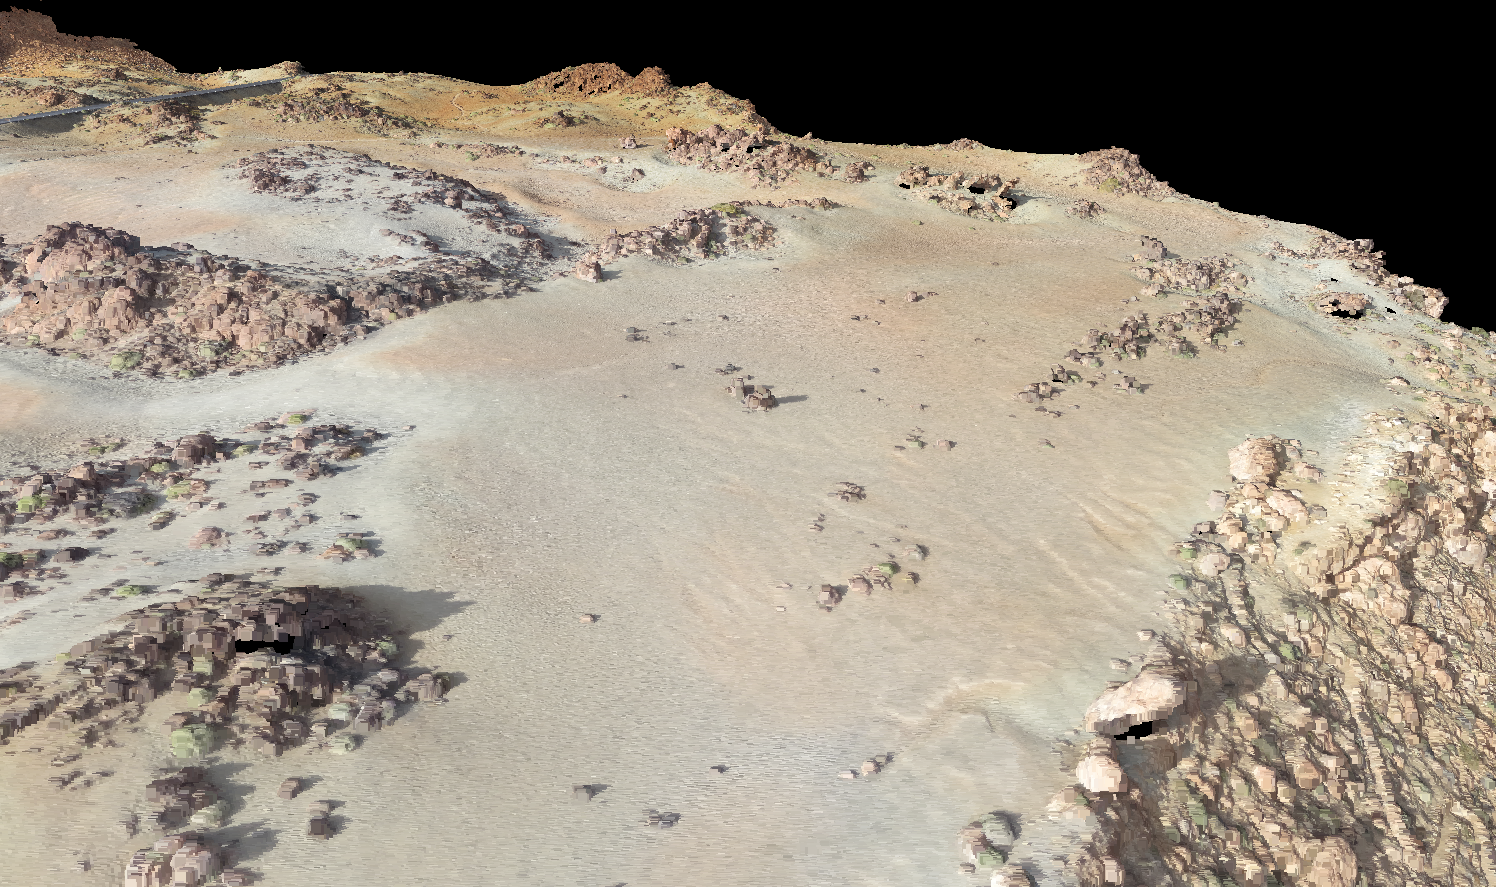
\includegraphics[scale=0.25]{terrain_2}
    \caption[Terrain of second experiment]{
        3D view of the terrain evaluated in the second experiment.
    }
    \label{fig:terrain_2}
\end{figure}

\begin{figure}[h!]
    \centering
    \begin{subfigure}{0.5\textwidth}
        \centering
        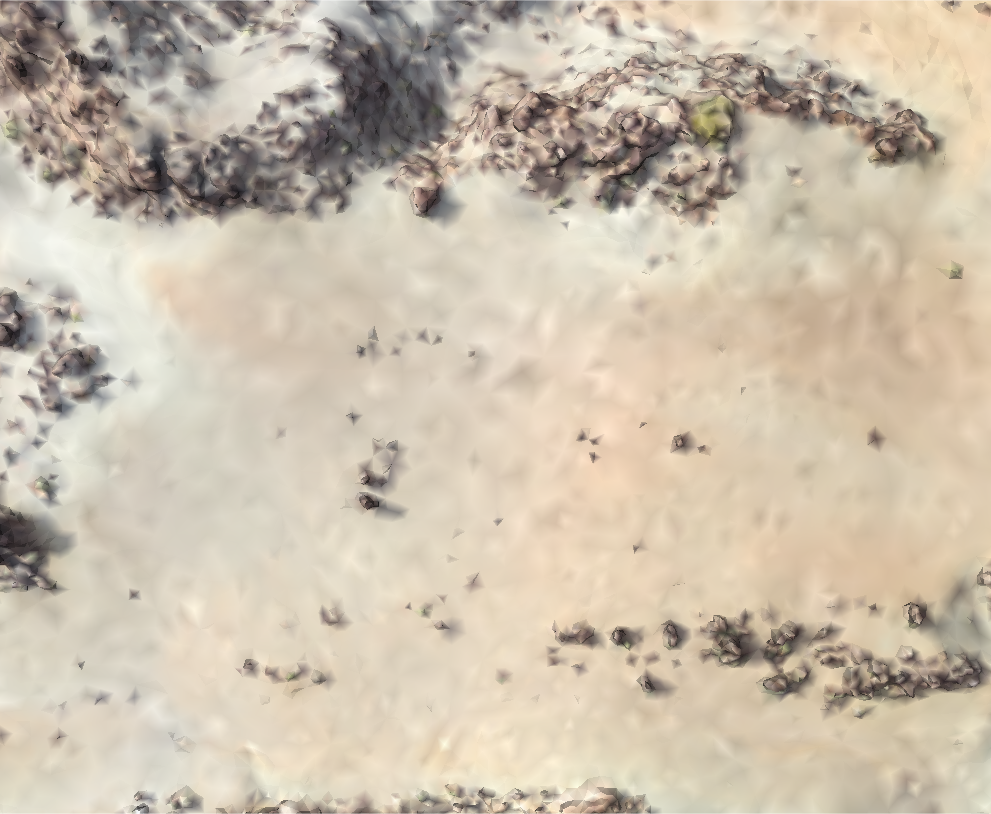
\includegraphics[scale=0.2]{bird_2_real}
        \caption{Point cloud projection}
        \label{fig:bird_2_real}
    \end{subfigure}
    \begin{subfigure}{0.5\textwidth}
        \centering
        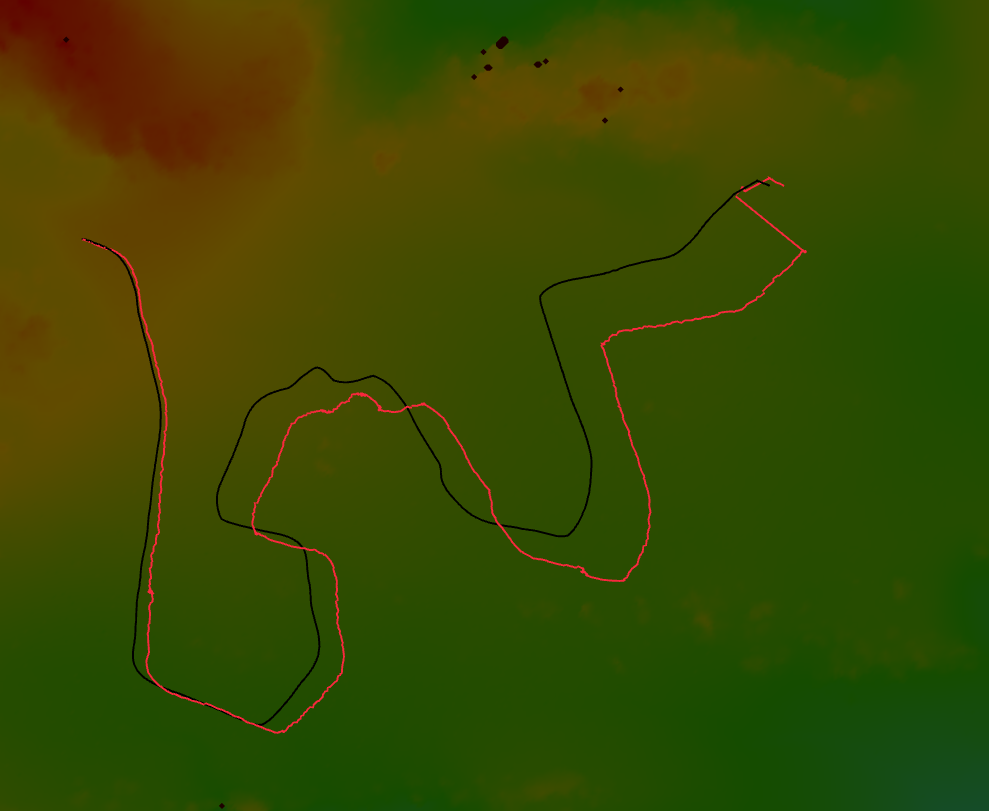
\includegraphics[scale=0.2]{bird_2_color}
        \caption{Global elevation map\\with an elevation colormap}
        \label{fig:bird_2_color}
    \end{subfigure}%
    \begin{subfigure}{0.5\textwidth}
        \centering
        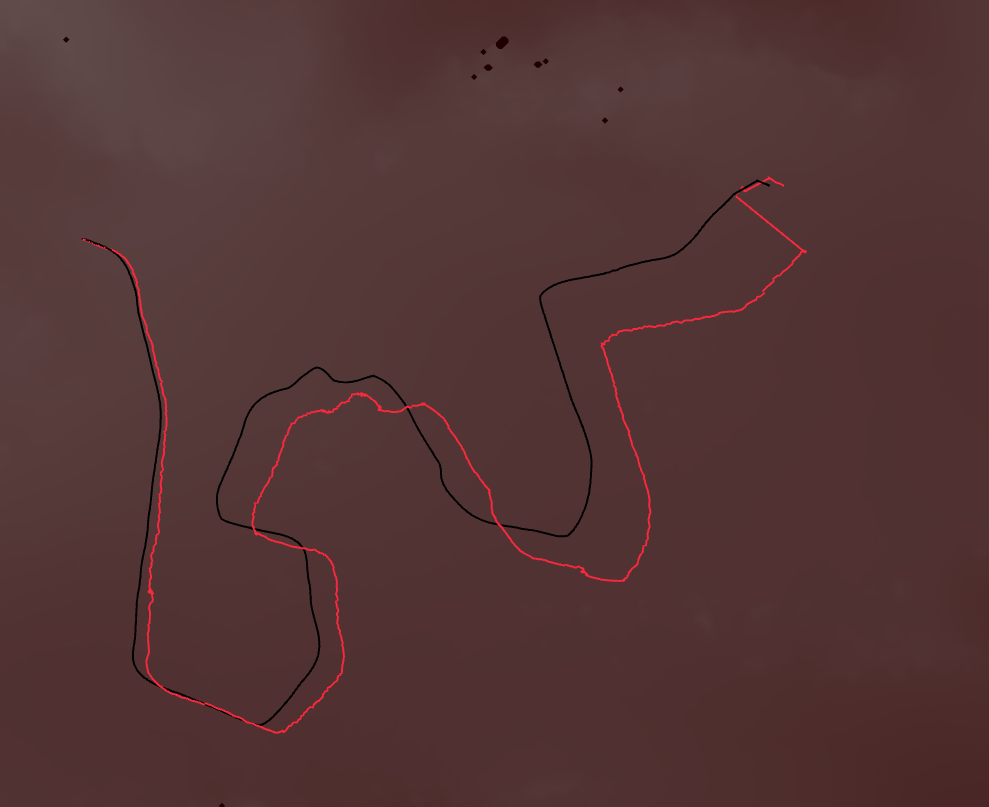
\includegraphics[scale=0.2]{bird_2_raw}
        \caption{Global elevation map\\with raw elevation values}
        \label{fig:bird_2_raw}
    \end{subfigure}
    \caption[Traverse of second experiment]{Orthographic views of the
        environment and the robot's traverses in it. The black and red colors
        correspond to the ground truth and SLAM paths accordingly. The pose
        correction is visible in the end of the traverse.}
    \label{fig:bird_2}
\end{figure}

In addition, we present the orthographic projections of the gradient of the
global elevation map (Figure \ref{fig:bird_2_global_gradient_map}) where
the elevation features are more visible.

\begin{figure}[h!]
    \centering
    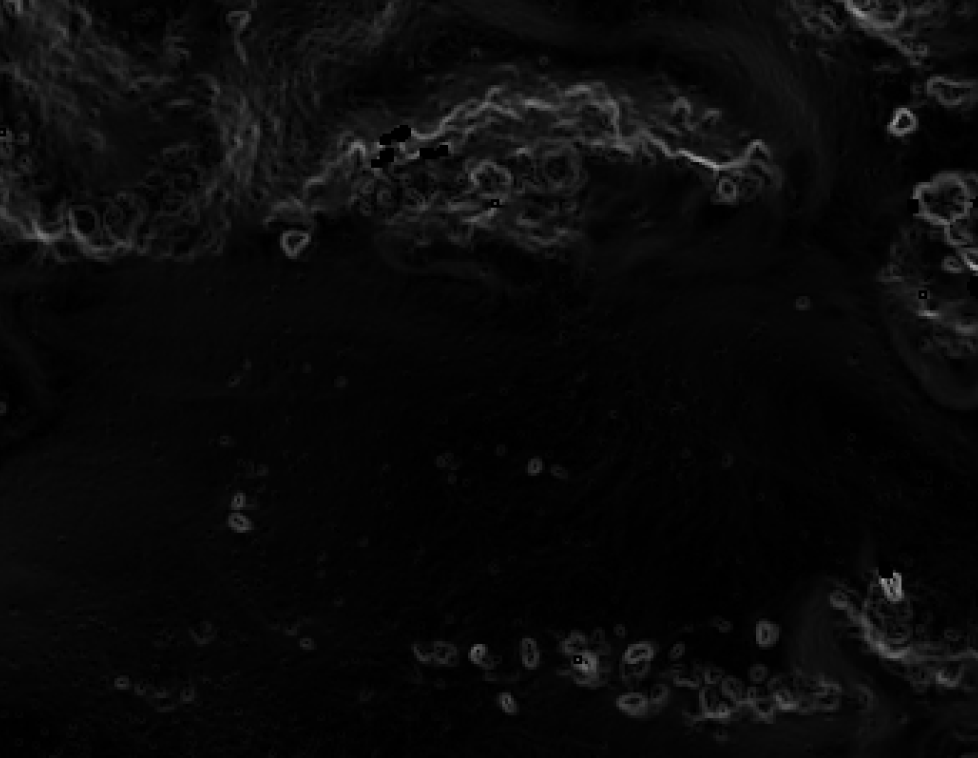
\includegraphics[scale=0.25]{bird_2_global_gradient_map}
    \caption[Global gradient map for pose correction]{
        The global gradient map that the local map is matched to for
        pose correction.
    }
    \label{fig:bird_2_global_gradient_map}
\end{figure}

The correction of the accumulated error is more visible in the plot of
Figure \ref{fig:pose_correction_error}.
The score of the yielded result from the global to local map matching,
as well as the rate of correction, are visible in Table
\ref{table:pose_correction}.
We can notice that the score of the match is $97.1\%$ (where $100\%$ is a
perfect match - as defined in Section \ref{map_matching}) and since
the matching threshold was set to $95\%$, the match is accepted and used
to correct the robot's pose by $98.6\%$.

\begin{figure}[h!]
    \centering
    \setlength\figureheight{8cm}
    \setlength\figurewidth{12cm}
    % This file was created by matplotlib2tikz v0.6.15.
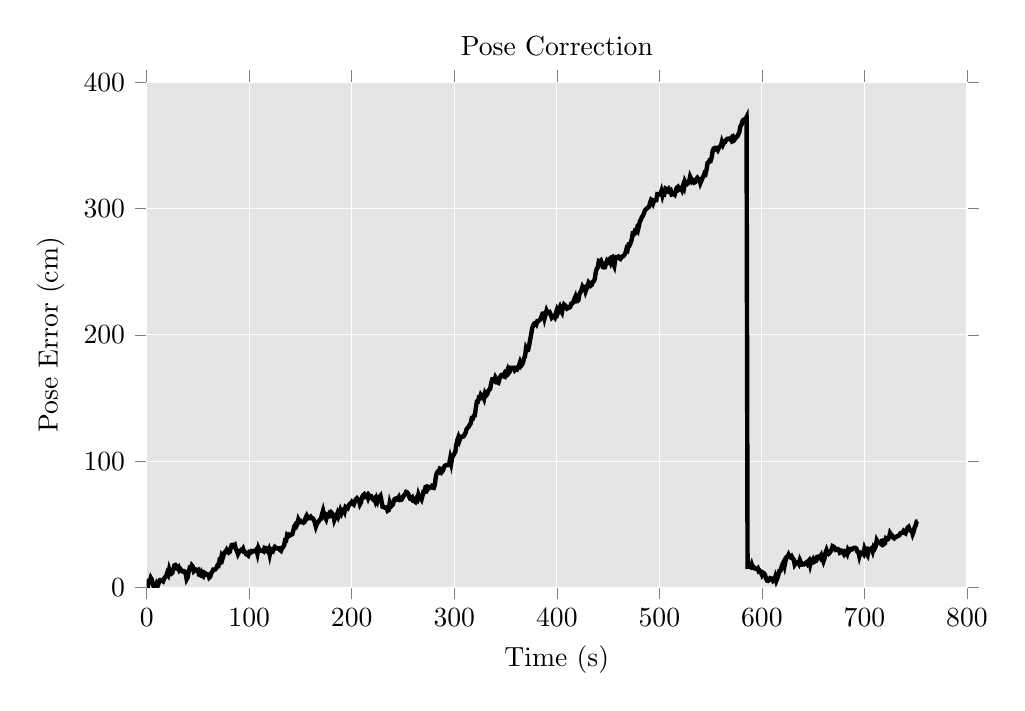
\begin{tikzpicture}

\begin{axis}[
title={Pose Correction},
xlabel={Time (s)},
ylabel={Pose Error (cm)},
xmin=0, xmax=800,
ymin=0, ymax=400,
width=\figurewidth,
height=\figureheight,
tick align=outside,
tick pos=both,
xmajorgrids,
x grid style={white},
ymajorgrids,
y grid style={white},
axis line style={white},
axis background/.style={fill=white!89.803921568627459!black}
]
\addplot [ultra thick, black, forget plot]
table {%
0 0.04124897123987
1 0.158133638850802
2 4.93982056138012
3 4.73535103639405
4 7.72278158142425
5 6.33771960300604
6 3.16242385231155
7 0.110979328246189
8 0.0798683868917822
9 0.344522637302146
10 3.1977214632242
11 1.91980181389725
12 4.12878420969794
13 5.89029260451897
14 5.82238239111087
15 5.55020881551674
16 4.95991022887759
17 7.1292105453959
18 8.25945394908929
19 9.11830200634492
20 11.4903874779837
21 10.1241491266426
22 14.3757967771083
23 11.8543354144067
24 11.0037119412718
25 11.6600427161706
26 14.207234753543
27 17.5354084105699
28 17.8747455293326
29 16.812720518545
30 15.4757590419027
31 16.3033448565468
32 13.6653114467488
33 14.4694956833645
34 13.291536102392
35 12.7655794747352
36 13.0456781404397
37 12.71185078537
38 11.0006527079467
39 6.65808296033092
40 8.17136470405908
41 12.4554697132398
42 15.3991410493046
43 15.009303891914
44 17.5847459644983
45 16.6143885325939
46 12.8550959731355
47 13.548576975412
48 14.1066317137672
49 13.4656137612441
50 13.9240689698234
51 10.2059484492881
52 9.8326500924238
53 11.6707203688083
54 9.45513806025263
55 8.86754383592853
56 11.8919325980059
57 11.4376626576107
58 10.2665777986181
59 10.5201904201853
60 10.1921492274878
61 7.88985846161079
62 8.64899865710527
63 11.4958555550706
64 12.453997528701
65 14.2465253297299
66 14.1761738119656
67 14.3752358169586
68 15.5165381201999
69 17.4544262178017
70 17.2356774938912
71 21.2873976859442
72 20.6970102175926
73 24.6277697306494
74 22.9171821419236
75 25.7700750413847
76 27.8534087752425
77 28.2036299789368
78 29.8182478542285
79 28.4123780599649
80 27.6203681167582
81 28.3327943138496
82 31.477046978349
83 33.703171306496
84 33.7655899763442
85 32.9912994892879
86 33.6767836197189
87 30.2395472996836
88 28.9595299078835
89 26.5681893293534
90 28.2428323634735
91 28.9909053933787
92 29.8019528396172
93 29.3727626745149
94 30.6841980809903
95 28.1220591729089
96 27.9709208654486
97 26.4182400947457
98 26.1193617995213
99 25.4248627653433
100 27.9762713777977
101 27.5662413463195
102 28.7497190239303
103 28.3297895344041
104 28.995254674578
105 29.0366628451603
106 28.6252248652751
107 29.8861233935867
108 26.8187514061725
109 31.235827300298
110 29.4275847767536
111 29.101338439819
112 29.3363936538024
113 29.2131742228972
114 28.6644105383136
115 31.4769710168024
116 31.2218585720627
117 29.3371930326733
118 28.4777512974469
119 30.1573317259947
120 26.1741431097239
121 30.1235627878241
122 29.336692546877
123 28.769524146598
124 30.8111842707483
125 32.2048251532349
126 31.5631263477756
127 30.9010689900678
128 30.9009151892862
129 31.0754921314943
130 29.7938509282377
131 29.1177413644454
132 31.3126021315477
133 32.0171848391263
134 33.2615151176493
135 37.3444278567124
136 37.2455571473542
137 41.5721323718548
138 40.7706529047399
139 41.857431825277
140 41.3514161453129
141 41.8983385910223
142 42.2079847928835
143 45.1412039926713
144 48.3435893026227
145 49.6962181974197
146 48.6352117872116
147 50.3304027574511
148 54.0088139594116
149 52.5691379270481
150 52.7907469018366
151 51.7747787365858
152 51.9581839565985
153 51.3994375891172
154 52.0540003161894
155 55.2636110540298
156 56.7934512074318
157 54.9669856551
158 55.7118777094223
159 55.2194942686886
160 56.0055537885755
161 54.8806985047696
162 54.7340123948254
163 53.7035151078816
164 51.3131660453994
165 48.2307948114676
166 50.4143485719789
167 51.5932851849023
168 52.5686446394359
169 53.9354270247145
170 54.4166369585
171 58.1937377468349
172 60.8824311671038
173 57.396597063068
174 55.6926675806636
175 54.1109474907171
176 57.3722342346116
177 56.8116157094581
178 58.4812866945937
179 57.5553927529018
180 59.3581807771865
181 58.4802444137397
182 57.6543928789382
183 53.4284063999228
184 55.4183580145675
185 56.566457226623
186 58.6927123218339
187 56.191075803207
188 58.1776785045979
189 61.1475287743787
190 59.0946822363935
191 61.2582624416391
192 61.7960674978925
193 60.0532846502286
194 63.8380384119157
195 63.2953597787002
196 62.7125481813297
197 64.6294300930519
198 66.1171302789809
199 66.2231197978899
200 67.5752606300245
201 66.4901436468017
202 65.7469615292813
203 68.2785719549667
204 69.8438526144031
205 70.6163086756569
206 69.4571716808953
207 69.2283725385675
208 65.9488687978247
209 67.4448765301052
210 71.369938844596
211 72.9852862314413
212 73.6905754351929
213 71.724883362574
214 72.0215220996209
215 73.0104924040534
216 70.7123541650291
217 72.7827336929669
218 71.6549667140341
219 71.9901801286091
220 70.4182940082935
221 69.6563309640263
222 70.4635608005672
223 68.2077371577449
224 70.6074864612957
225 68.4963581496138
226 71.4182002435511
227 71.7489662548311
228 72.6969959207809
229 68.5044120446886
230 64.0290099253766
231 63.9287302115731
232 63.3079013137878
233 63.1851671628983
234 63.4381545993889
235 60.8224280439698
236 61.3277258218562
237 66.6123655387249
238 63.8521860686968
239 64.6616068903157
240 65.6004251530302
241 68.6746820919694
242 70.1470550103061
243 70.4822020004291
244 69.6321046716745
245 69.976227091137
246 71.511779631289
247 69.2847572988783
248 69.3120038065205
249 70.0218822401101
250 71.8469642668372
251 72.9978204741204
252 73.9107836805613
253 75.6545377902187
254 75.3022057127238
255 74.3428510347275
256 71.8945899702792
257 70.250957304087
258 70.3728826005901
259 71.1919631688778
260 68.5576947512005
261 68.4292037736388
262 67.7963803204841
263 70.136644726756
264 69.3670982501702
265 73.4704127276499
266 71.1912501949335
267 70.9079187509572
268 69.6404176216524
269 72.6144256643876
270 75.8690002467269
271 75.7827204736189
272 79.67290113678
273 79.8947036841097
274 77.7662873322173
275 79.0232236018854
276 79.4916161174246
277 79.2297800382331
278 80.187983656663
279 79.1669753548153
280 78.9074299267993
281 81.2589846565209
282 87.6173149784718
283 90.8387838679856
284 91.8431409451788
285 91.3828597249169
286 94.0612468305374
287 93.6523382435316
288 91.7110974721968
289 92.7525780140632
290 95.4266926245609
291 96.5291462943153
292 96.9132904962521
293 96.9609662406895
294 96.9069302323009
295 97.7529191877481
296 102.038363354117
297 98.4190042663378
298 103.065759190065
299 104.610597409562
300 105.984669736673
301 107.384945439045
302 113.087092311613
303 116.688165204085
304 118.944597645334
305 116.390341792033
306 118.678961614997
307 119.440741792148
308 119.335915830667
309 119.63492656561
310 120.973156034206
311 122.445096828612
312 125.452025288498
313 126.325364180062
314 127.208204296644
315 128.79741095371
316 129.926875362953
317 133.896441123211
318 133.783655915825
319 135.96285844988
320 136.27135043871
321 142.149978783732
322 146.974495826883
323 147.017000486417
324 150.325784501644
325 150.090209754737
326 152.886501619246
327 152.044784491333
328 151.3087730832
329 149.417192929413
330 153.498246241993
331 151.95905083518
332 152.837032369335
333 155.278844400349
334 156.581944628571
335 157.295416093534
336 161.893238644575
337 164.761198784353
338 164.620410932653
339 163.795325702452
340 166.344637021936
341 164.818374097113
342 162.371046575064
343 162.018054426094
344 164.912712435873
345 167.113257129464
346 168.290866211919
347 168.383631223872
348 167.644443632598
349 169.419693106735
350 168.044278823335
351 170.060987607841
352 172.254170994879
353 169.663901293898
354 170.705293337073
355 173.93817796975
356 173.848765590612
357 173.87976146455
358 173.952733780171
359 172.042804313498
360 172.922794755849
361 172.603293591899
362 174.650348469692
363 175.339936645744
364 177.928511016597
365 175.367070766131
366 176.270029227835
367 178.072612181551
368 181.337107158146
369 183.18125420852
370 189.287305601743
371 187.688078333704
372 188.013747631917
373 191.836350103677
374 196.309779115973
375 200.484151654234
376 205.55090058601
377 207.537378686112
378 209.041102757612
379 209.392015720556
380 208.340942345118
381 210.857400397259
382 210.923752017535
383 211.550196507697
384 212.74853898236
385 214.466670839981
386 216.791351464971
387 216.920876225044
388 213.088366914957
389 216.181743775751
390 219.228855487186
391 217.511711407929
392 217.16609488368
393 217.780715073617
394 216.147794993089
395 213.687123674759
396 214.594307041925
397 214.7018729285
398 213.717012679665
399 217.23925637571
400 219.646830292464
401 217.424708283483
402 219.56860082469
403 221.678157461759
404 219.163831062928
405 217.750508550304
406 222.021846990639
407 224.091042666688
408 223.327626004184
409 222.49519395127
410 220.829492562236
411 221.338662360163
412 221.508276471798
413 222.023183178448
414 224.652875557719
415 224.849526303605
416 225.776438041245
417 228.101873180804
418 230.045474211281
419 226.572674237477
420 226.655207755145
421 227.455541258732
422 232.167787998381
423 233.706966458734
424 235.474915787369
425 238.0871859257
426 236.657366477378
427 237.313909460145
428 234.309833199607
429 236.478323567195
430 238.55055372669
431 241.30491205527
432 240.291238987844
433 238.910763678485
434 239.523705571939
435 242.006748388787
436 242.551748943584
437 244.228817850255
438 249.812945495181
439 252.567937675924
440 253.478010814081
441 258.341061558361
442 257.959716003391
443 258.781129645413
444 256.653238434352
445 253.616055386296
446 253.369548923597
447 253.55839808748
448 256.948211643795
449 258.902030056893
450 258.069904880596
451 259.248435832523
452 257.470887145067
453 261.181675218814
454 261.605311797252
455 256.257366137848
456 254.393577649753
457 259.716822346376
458 261.593860301549
459 261.585179952253
460 261.922200706467
461 260.642644360576
462 260.117089021851
463 261.375656357909
464 262.169384513264
465 262.34440111657
466 263.439844230603
467 265.061195174156
468 268.165081736391
469 267.355109367445
470 271.281878081497
471 271.051821848169
472 272.945679456676
473 275.431613810428
474 280.013699875074
475 279.760443413054
476 282.009429260889
477 281.491228688965
478 284.052598845266
479 282.667351175286
480 286.106438211656
481 289.96450324926
482 290.953616688769
483 293.504961271334
484 294.286386580479
485 296.389787813107
486 298.728156381967
487 299.486285671219
488 300.165676518096
489 300.968967795328
490 301.434534997265
491 304.924946349871
492 307.074998881053
493 306.494140888578
494 304.310518721176
495 306.480892034038
496 306.595101655581
497 306.624683718868
498 311.435632622984
499 311.369109139841
500 311.248333170053
501 311.204967035083
502 313.749756291204
503 310.314118040476
504 313.080598669806
505 312.238106472163
506 315.759535308196
507 315.27140179725
508 314.277804637565
509 315.386606411861
510 313.647077617174
511 314.278700458736
512 311.087838460037
513 311.316517045081
514 312.004439092398
515 311.175581885356
516 314.235617640429
517 316.540419867933
518 317.160660414191
519 315.197226473823
520 315.973939086793
521 316.379471527477
522 314.700813392391
523 317.757135821478
524 316.227432334347
525 321.39324853969
526 319.83569585186
527 319.333177893926
528 319.991640473627
529 321.307872083846
530 325.282692231792
531 323.56397510947
532 321.134996003505
533 321.727582518273
534 320.494442154818
535 320.956026532712
536 323.412621057247
537 324.309175498796
538 323.049688216278
539 323.179840729874
540 320.13010743252
541 322.046112876358
542 323.944526443041
543 325.531445773141
544 327.857810570294
545 327.317617399264
546 330.840682385866
547 336.106541395544
548 336.463697777676
549 338.067686371129
550 337.837132502694
551 340.512345053886
552 345.621221393582
553 347.438037307388
554 347.850951652382
555 347.047441346415
556 347.548056524063
557 346.248852537739
558 347.956427459902
559 349.095556046648
560 349.463676419937
561 352.780451471813
562 350.634694042916
563 352.464833911306
564 352.579007724566
565 354.142046908028
566 355.027379567306
567 355.301001334714
568 355.372412099057
569 354.654560367082
570 355.66914235712
571 353.059776408188
572 353.395179462015
573 356.309555891894
574 355.419711869507
575 356.698457714954
576 356.98000822062
577 358.685956322476
578 360.535507023368
579 364.867672990031
580 366.191807740499
581 369.006476696498
582 370.260598918031
583 370.628380998854
584 370.725862790329
585 372.31302607838
586 16.492701268878
587 16.584039370043
588 16.572103075558
589 16.14942788627
590 18.380607708281
591 15.887983480942
592 16.131354901272
593 15.17201073589
594 15.118320319766
595 14.574691507875
596 15.28150438046
597 12.836897933233
598 13.225077553248
599 12.155533362968
600 10.16348070705
601 11.81239871239879
602 11.29094883988598
603 10.1804353276434
604 7.07713867483699
605 5.56710176984099
606 5.32712557937183
607 6.02738670636566
608 7.41214944952083
609 7.15979409030508
610 7.05089947549582
611 5.18195992503131
612 5.73022758039179
613 8.32896679019847
614 5.31685440268382
615 7.2551470190415
616 9.97715930921886
617 13.0910423249655
618 13.3074007324508
619 15.7899939214104
620 18.2645599902738
621 19.8529016850455
622 17.0204648993605
623 21.2556505605186
624 24.0385533601041
625 24.258650602062
626 25.982192537513
627 24.2677242997322
628 23.8195854054925
629 24.7086747514898
630 23.0487956129428
631 22.3353364599343
632 18.1910682037371
633 19.3784889546316
634 19.7512064450682
635 20.1067781925781
636 18.8138861485794
637 21.7973245554438
638 19.9994264480011
639 18.2063549685619
640 18.3028402475788
641 18.3402744857949
642 19.1170758024805
643 19.7014734103276
644 18.7259447578756
645 20.5482683559464
646 21.5174337139301
647 18.0143879634852
648 21.4003919919752
649 20.7159363527445
650 22.2630263556385
651 20.3757458010509
652 20.8639674109439
653 21.1938809230695
654 24.2944877000714
655 24.2562355293848
656 24.7476844263881
657 23.5474755069272
658 25.3564457195877
659 23.1028629332768
660 20.7358514825321
661 23.0461286383084
662 27.5565818537279
663 29.6612845486981
664 27.4082995194716
665 26.6323135250469
666 27.4825919635415
667 28.6467454485792
668 30.0489237713246
669 32.7428076944582
670 32.3314361988735
671 31.3960954758739
672 29.8662891774293
673 30.1725657845716
674 30.4893049661763
675 29.9831458262664
676 27.6001394148343
677 28.0076777430924
678 28.8558809195517
679 28.2278440105353
680 26.6973305450566
681 28.453730801022
682 27.9233970468058
683 26.491744361213
684 30.0628069147843
685 28.8766568128441
686 30.1868154169105
687 30.6508163597951
688 30.2727469197397
689 30.9358732140536
690 31.4554406530986
691 31.4061992905045
692 30.9993633806429
693 28.5794025443801
694 28.2401170429332
695 24.7122324648796
696 27.664454625127
697 27.4586881954538
698 27.4106117343922
699 26.4747038236087
700 30.6792185844829
701 28.5356559718526
702 26.7886642396121
703 25.5523518230925
704 30.5844175602634
705 30.283951827617
706 30.0156964286215
707 30.9205260774635
708 28.633058175622
709 32.0422002754426
710 31.0122116418066
711 32.6958113064406
712 37.5315516973999
713 36.1505112621629
714 35.891914784548
715 35.3679501910541
716 34.6566275945304
717 37.056508063777
718 37.259450102141
719 34.4240904625514
720 35.0102734459756
721 38.6582448865623
722 37.9678769471078
723 38.2415052051212
724 39.6932237225209
725 43.11703002498
726 41.8551864832097
727 41.3242082309062
728 39.5646445457947
729 38.9762524795831
730 39.9542032037691
731 40.0367874462137
732 40.7035194532698
733 40.9853263428807
734 41.345687755889
735 42.8501436924307
736 43.2275716289841
737 43.4140235666453
738 44.6419033149519
739 43.5600031175617
740 42.9575895496936
741 44.8585003472796
742 47.3835176056166
743 48.0348652689983
744 45.903411789393
745 45.0581449931934
746 45.061548840781
747 42.2861439714532
748 44.3817259688104
749 47.7816261893772
750 49.3132844429109
751 52.2643970861412
752 52.4541249289298
};
\end{axis}

\end{tikzpicture}

    \caption[Pose correction error over time plot]{
        Pose correction results of second experiment.
    }
    \label{fig:pose_correction_error}
\end{figure}

\begin{table}[h!]
    \centering
    \begin{tabular}{| c | c |}
        \hline
        Execution time of one iteration of matching &
            $\SI{630}{\milli\second}$ \\
        \hline
        Total execution time of matching & $\SI{12.6}{\sec}$ \\
        \hline
        \hline
        Percentage of correction in position & $98.6\%$ \\
        \hline
        Percentage of correction in orientation & $82.9\%$ \\
        \hline
        \hline
        Score of the matched location & $97.1\%$ \\
        \hline
        Acceptance threshold of match & $95\%$ \\
        \hline
    \end{tabular}
    \caption[Results of pose correction for absolute localization]{
        Resulting time, correction and score of the match found.
    }
    \label{table:pose_correction}
\end{table}

As we already mentioned, the exact moment of correction is determined by
the two criteria that were defined in the implementation of the Pose Correction
module (see Section \ref{pose_correction_criteria}).
However, since both of them are straightforward, their experimental
validation is left out.

\subsection{Map Resolution Viability}

In this experiment, we validate and measure the performance of our map
matching technique for absolute localization by performing the same
scenarios with different combinations of resolutions for the local and
global maps.
This is done with the aim to draw conclusions regarding the viability
of our approach with respect to the available global map data as well as
the processing capabilities of a robot.

Figure \ref{fig:global_map_resolution} presents the local and global elevation
maps with distinct resolution values.
Upon matching these maps, we observe the score of each match for every
combination of resolutions (Table \ref{table:map_resolutions}).
We can notice that a low resolution global map has more impact in the map
matching score than a low resolution local map.
In fact, a global map with a resolution of $\SI{2.0}{\m \per pixel}$ yields
poor results for every resolution of the local map.
On the other hand, a global map with a resolution of $\SI{1.0}{\m \per pixel}$
has the possibility to yield a high score only when the resolution of
the local map is high enough.

\begin{figure}[h!]
    \centering
    \begin{subfigure}{0.5\textwidth}
        \centering
        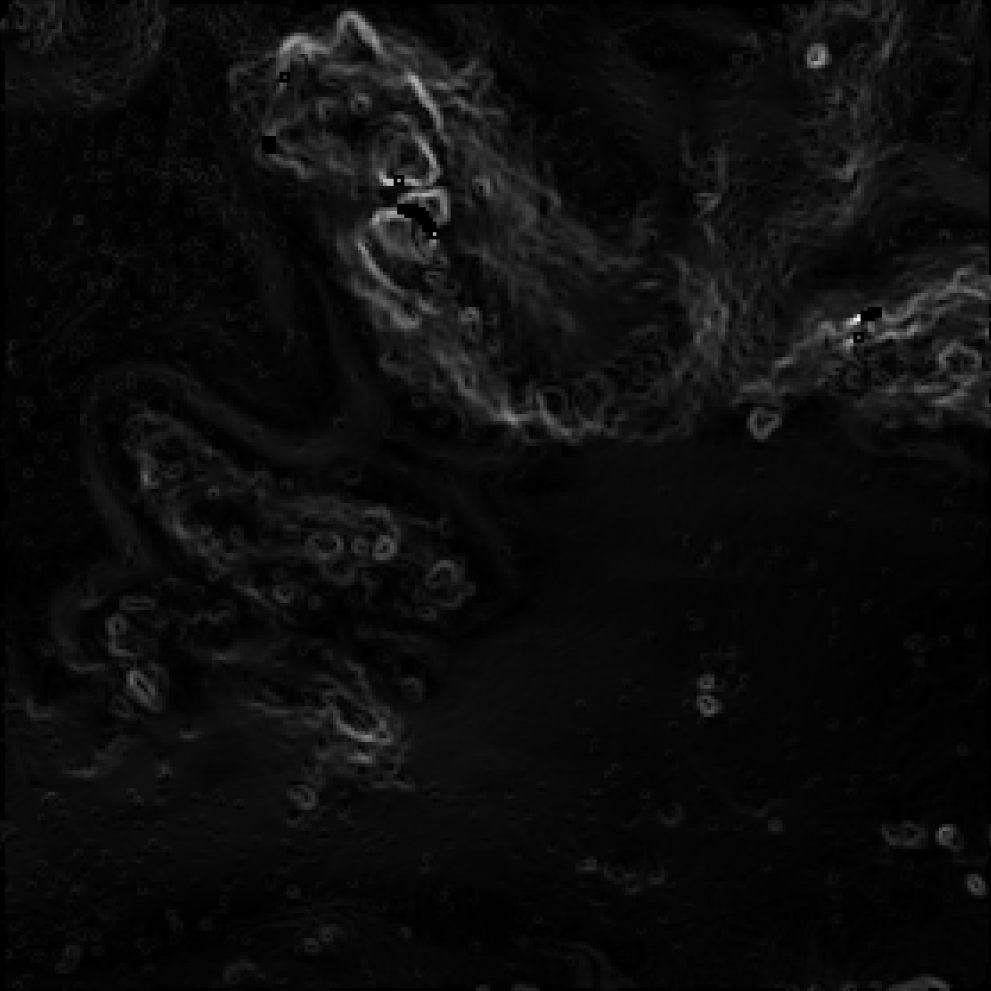
\includegraphics[scale=0.175]{global_resolution_1}
        \caption{}
        \label{fig:global_resolution_1}
    \end{subfigure}
    \begin{subfigure}{0.5\textwidth}
        \centering
        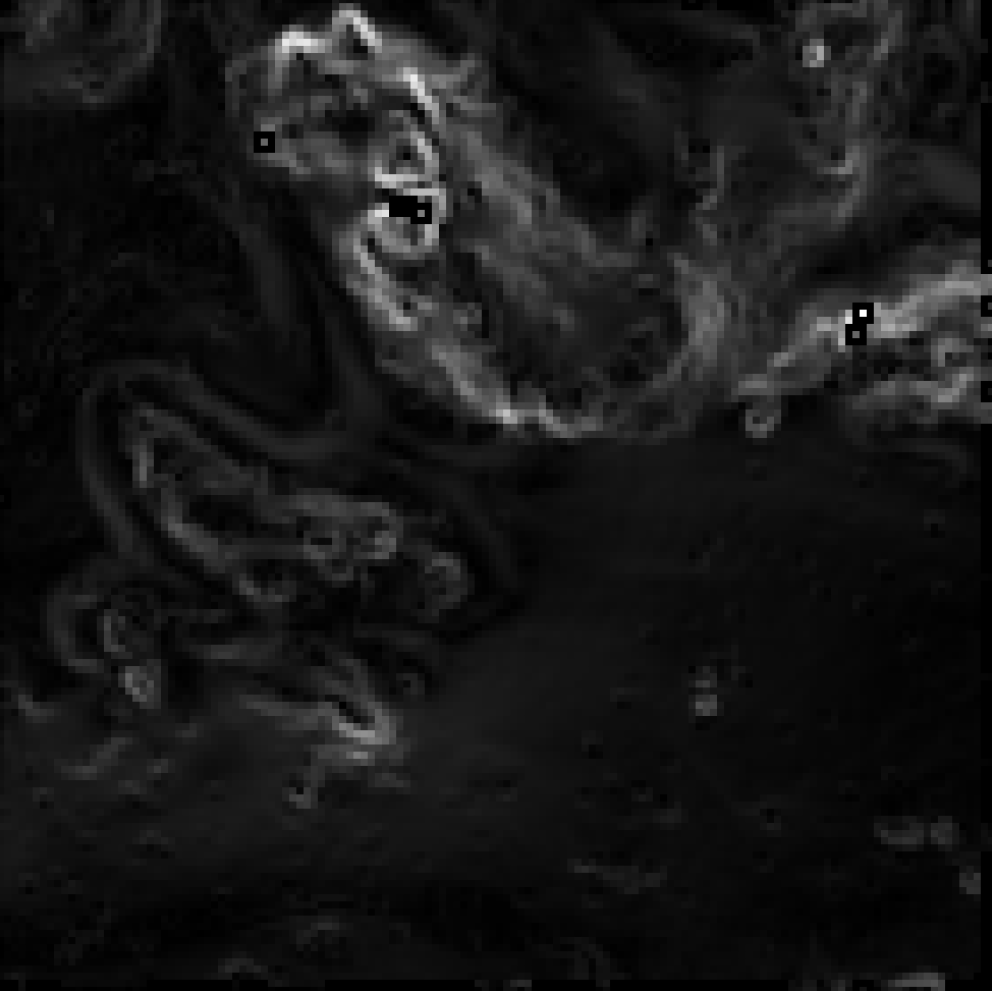
\includegraphics[scale=0.175]{global_resolution_2}
        \caption{}
        \label{fig:global_resolution_2}
    \end{subfigure}%
    \begin{subfigure}{0.5\textwidth}
        \centering
        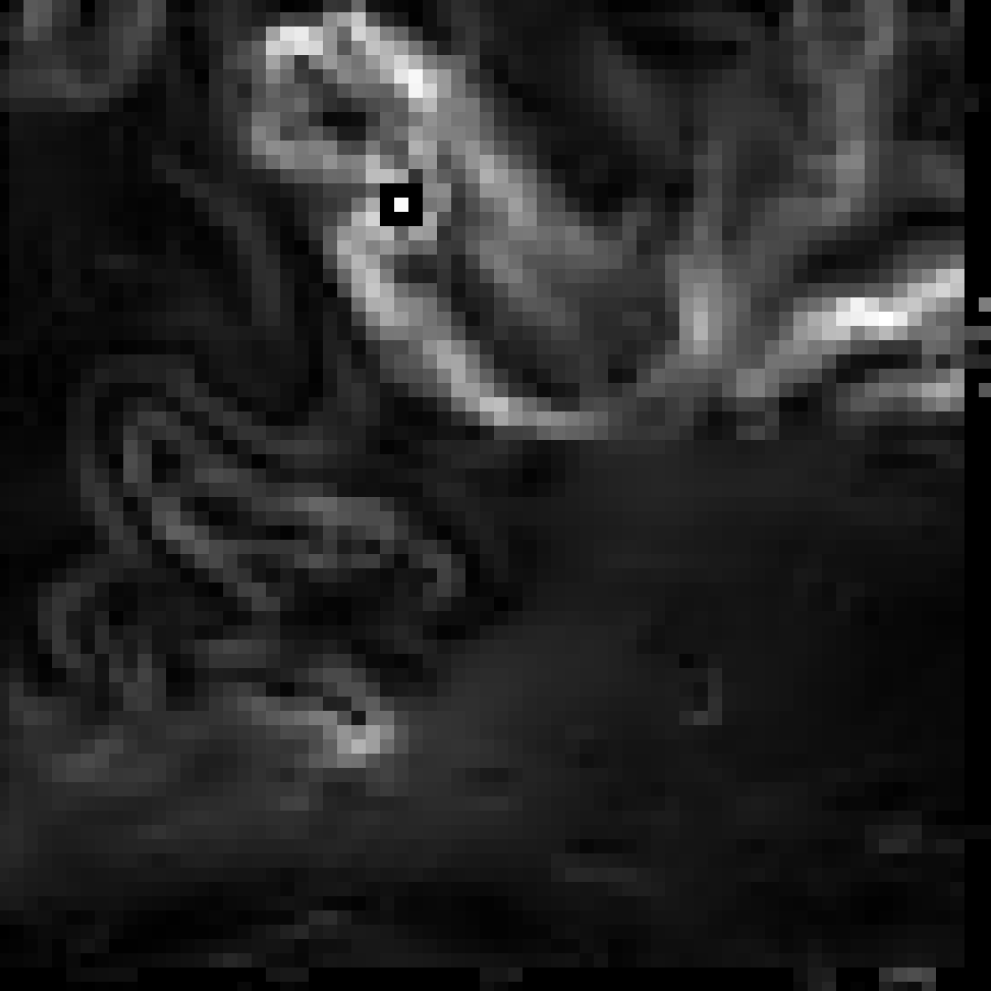
\includegraphics[scale=0.175]{global_resolution_3}
        \caption{}
        \label{fig:global_resolution_3}
    \end{subfigure}
    \caption[Global map resolution comparison]{Comparison of global gradient
        map resolution.
        (a) Resolution of $\SI{0.5}{\m \per pixel}$.
        (b) Resolution of $\SI{1.0}{\m \per pixel}$.
        (c) Resolution of $\SI{2.0}{\m \per pixel}$.
        }
    \label{fig:global_map_resolution}
\end{figure}

\begin{table}[h!]
    \centering
    \begin{tabular}{| c | c || c |}
        \hline
        Local map & Global map & Matching \\
        resolution (m) & resolution (m) & score \\
        \hline
        \hline
        0.1 & 0.5 & $97\%$ \\
        \hline
        0.1 & 1.0 & $76\%$ \\
        \hline
        0.1 & 2.0 & $48\%$ \\
        \hline
        \hline
        0.2 & 0.5 & $91\%$ \\
        \hline
        0.2 & 1.0 & $67\%$ \\
        \hline
        0.2 & 2.0 & $32\%$ \\
        \hline
        \hline
        0.5 & 0.5 & $72\%$ \\
        \hline
        0.5 & 1.0 & $36\%$ \\
        \hline
        0.5 & 2.0 & $25\%$ \\
        \hline
    \end{tabular}
    \caption[Local and global map resolution viability]{
        Score of match for combinations of local and global map resolutions.
    }
    \label{table:map_resolutions}
\end{table}

Although the size and resolution of the local map are parameters that we
determine, they are highly limited by the on board processing power of the
robot, since the higher the resolution the more computations must be performed.
On the other hand, the resolution of the global map is a parameter that is
determined by the equipped camera sensors of the orbiters and the
reconstruction techniques applied to the imagery received from those.
As the technology of the space industry advances, we can expect to observe
in the next few years an increase in the aforementioned resolution parameters
and, consequently, an increase in efficiency of the map matching techniques.
As an example, the HiRISE on board camera of the
\textit{Mars Reconnaissance Orbiter} can currently achieve a resolution of
$\SI{30}{\cm \per pixel}$ with the possibility to acquire stereo image pairs
with a precision better than $\SI{25}{\cm \per pixel}$ over locations of
high priority, i.e. potential landing site of future missions to Mars.

